% =====================================================================
%  Splitting Orders Across AMM Pools with CVaR Execution-Risk Control
%  Convex Optimization - Project 3 report
%  Compile: latexmk -pdf main.tex
% =====================================================================
\documentclass[11pt,a4paper]{article}

\usepackage[T1]{fontenc}
\usepackage[utf8]{inputenc}
\usepackage{lmodern}
\usepackage{microtype}
\usepackage[margin=2.6cm]{geometry}
\usepackage{graphicx}
\usepackage{booktabs}
\usepackage{array}
\usepackage{amsmath,amssymb,amsthm,bm}
\usepackage{xcolor}
\usepackage{fancyhdr}
\usepackage{caption}
\usepackage{subcaption}
\usepackage{listings}
\usepackage{enumitem}
\usepackage{algorithm}
\usepackage{algpseudocode}
\usepackage{pdflscape}
\usepackage{float}
\usepackage{placeins}
\usepackage[colorlinks=true,linkcolor=blue!50!black,citecolor=blue!50!black,urlcolor=blue!50!black]{hyperref}

\graphicspath{{../results/figures/}}
\captionsetup{font=small,labelfont=bf}

\pagestyle{fancy}
\fancyhf{}
\fancyhead[L]{\small AMM Order Splitting with CVaR}
\fancyhead[R]{\small Convex Optimization -- Project 3}
\fancyfoot[C]{\thepage}
\setlength{\headheight}{14pt}

\newtheorem{proposition}{Proposition}
\newtheorem{lemma}{Lemma}
\theoremstyle{remark}
\newtheorem{remark}{Remark}

\lstdefinestyle{pystyle}{
  language=Python,
  basicstyle=\ttfamily\footnotesize,
  breaklines=true,
  showstringspaces=false,
  keywordstyle=\color{blue!60!black}\bfseries,
  commentstyle=\color{green!40!black}\itshape,
  stringstyle=\color{orange!80!black},
  numbers=none,
  frame=single,
  rulecolor=\color{black!25},
  tabsize=4
}
\lstdefinestyle{logstyle}{
  basicstyle=\ttfamily\scriptsize,
  breaklines=true,
  breakatwhitespace=false,
  columns=fullflexible,
  keepspaces=true,
  frame=single,
  rulecolor=\color{black!25},
  numbers=none
}

\newcommand{\cvar}{\texorpdfstring{\ensuremath{\mathrm{CVaR}}}{CVaR}}
\newcommand{\var}{\texorpdfstring{\ensuremath{\mathrm{VaR}}}{VaR}}
\newcommand{\E}{\texorpdfstring{\ensuremath{\mathbb{E}}}{E}}
\newcommand{\code}[1]{\texttt{#1}}

\title{\textbf{Splitting Orders Across AMM Pools\\
with CVaR Execution-Risk Control}\\[0.6em]
\large Convex Optimization -- Project 3\\
(Assignment topic: Order Splitting Between AMMs with Tail-Risk Reduction)}
\author{Parham Moshashaei \quad (Student ID: 402111389)}
\date{September 2026}

\begin{document}

\maketitle
\thispagestyle{empty}

\begin{abstract}
\noindent
A large sell order on decentralized exchanges suffers quadratic price impact, pays fixed gas
for every pool it touches, and faces uncertain pool depth at execution time.  This report
studies the convex optimization problem of splitting an order of size $F$ USD across $M$
automated-market-maker (AMM) pools with execution-cost risk measured by Conditional
Value-at-Risk (\cvar{}), following the project statement exactly: convex cost
$c_m(f_m) = a_m f_m + b_m f_m^2/L_m$ derived from the constant-product invariant $xy=k$,
scenario liquidity $L_{m,k}=L_m(1-\delta_{m,k})$, fractional pool-usage variables $z_m$, and
the objective $\frac{1}{K}\sum_k C_k(f) + \lambda\,\cvar_\alpha(C)$.

All experiments use \textbf{real market data}: 25{,}544{,}800 real ETH/USDT trades
(\$24.15B notional over 30 days, Binance), 2{,}500 real parent orders (\$1k--\$16.7M), and
the real TVL histories of five Ethereum USDC-WETH pools (Uniswap V3 at 0.05\%/0.3\%/0.01\%,
Uniswap V2, SushiSwap) from DefiLlama.  Scenario deviations are historical resamplings of
real TVL shortfalls against each pool's own typical level.

Headline results.  (i)~In-sample, the \cvar{} router (\(F=\$250\)k, $\alpha=0.95$,
$\lambda=1$) cuts $\cvar_{0.95}$ by \textbf{19.6\%} relative to the best single pool and
0.7\% relative to mean-only optimization.  (ii)~Out-of-sample, on a walk-forward backtest of
\textbf{2{,}500 real trades} with no look-ahead, it reduces realised tail cost by
\textbf{32.3\%} and mean cost by \textbf{\$3{,}078 per order} versus the best single pool,
with the advantage concentrated in orders above $F\approx\$100$--$200$k.  (iii)~\cvar{}
weighting is cheap insurance: tied with mean-only out of sample (0.1\% tail difference) but
strictly better under high liquidity uncertainty (3.5\% tail improvement at twice the
observed deviation intensity).  We also prove that the prescribed $z_m$ relaxation of the
binary pool-usage indicator collapses to $z_m=f_m/F$ (so the sparsity penalty
$\eta\sum_m z_m$ is constant), quantify the resulting relaxation gap, and correct 14 issues
of the earlier project notebooks (including fabricated ``real data'' claims and an inverted
scenario risk ordering).
\end{abstract}

\tableofcontents
\newpage

% =====================================================================
\section{Introduction and problem statement}
% =====================================================================

Decentralized exchanges execute trades against automated market makers (AMMs).  The price
impact of a trade grows with its size, every additional pool touched incurs a fixed gas
cost, and the effective depth of a pool at execution time is uncertain (liquidity migrates,
and transaction ordering introduces adverse selection).  The practical question studied in
this project is:

\begin{quote}
\itshape
Given $M$ AMM pools with liquidity indices $L_m>0$, fees $\phi_m\in[0,1)$ and fixed costs
$g_m\ge 0$, and a total order of size $F$ USD, how should $F$ be split across pools so as to
balance expected execution cost against tail (worst-case) execution cost, where pool depth
degrades by unknown amounts $\delta_{m,k}$ in adverse scenarios?
\end{quote}

The model prescribed by the project statement is a \emph{convex} surrogate of the exact AMM
cost curves, with \cvar{} (mean excess loss) as the risk measure and a fractional relaxation
of the binary ``is pool $m$ used'' indicator.  The main deliverables are:

\begin{enumerate}[leftmargin=2.2em]
  \item \textbf{Model description and parameter selection} -- justification of $L_m$,
        $\phi_m$, $a_m$, $b_m$ and of the scenario model $\delta_{m,k}$ (Section~\ref{sec:data}
        and Section~\ref{sec:model}; if real data is used, as here, the extraction must be
        explained).
  \item \textbf{Convexity analysis} -- convexity of the scenario costs $c_k(f)$ and of the
        \cvar{} reformulation (Section~\ref{sec:convexity}).
  \item \textbf{Numerical solution in CVXPY} -- problem dimensions $(M,K)$, solver name and
        solve time (Section~\ref{sec:numerics}).
  \item \textbf{Sensitivity analysis} -- sweeps over the confidence level $\alpha$, over the
        order size $F$ (from what point is splitting necessary?), and over the uncertainty
        intensity $\delta$ (how much does \cvar{} protect the plan?)
        (Section~\ref{sec:sensitivity}).
  \item \textbf{Baseline comparison} -- single-pool best and mean-only optimization
        (Section~\ref{sec:baselines}).
\end{enumerate}

Beyond the statement we add (i)~a validation of the cost-model shape on the real trade tape
(Section~\ref{sec:model}), (ii)~an out-of-sample \textbf{walk-forward backtest on 2{,}500
real trades} (Section~\ref{sec:backtest}), (iii)~an analysis of the $z_m$ relaxation
(Section~\ref{sec:relaxation}), and (iv)~a review of the earlier project notebooks and the
issues corrected (Section~\ref{sec:review}).

% =====================================================================
\section{Real data and parameter selection}
\label{sec:data}
% =====================================================================

Everything used below is either downloaded from public sources or derived from downloads by
stated formulas.  No number is invented and labelled as an observation.  Table~\ref{tab:provenance}
summarizes the provenance of every quantity.

\begin{table}[H]
\centering
\caption{Data provenance.  ``Real'' = downloaded observation; ``derived'' = computed from
real data by a stated formula; ``estimated'' = a documented assumption.}
\label{tab:provenance}
\small
\begin{tabular}{@{}p{5.2cm}p{5.0cm}p{2.2cm}@{}}
\toprule
\textbf{Quantity} & \textbf{Source} & \textbf{Status} \\
\midrule
Trade tape: 25{,}544{,}800 ETH/USDT trades, \$24.15B notional, 30 days
  (2026-08-16 to 2026-09-14) & Binance Vision daily \code{aggTrades} & real \\
Parent orders: 1-minute taker-sell notional, 2{,}500 orders & aggregated from the tape &
derived (aggregation only) \\
Pool TVL $V_m(t)$, daily, 2022--2026, 5 Ethereum USDC-WETH pools
  & DefiLlama \code{yields.llama.fi} chart API & real \\
Pool identity and fee tier & DefiLlama pool metadata + protocol constants & real \\
Liquidity index $L_m = \mathrm{TVL}_m/2$ & derivation from $xy=k$ (Section~\ref{sec:model}) &
derived \\
Cost coefficients $a_m=\phi_m$, $b_m=1$ & derivation from $xy=k$ + fees & derived \\
Scenario deviations $\delta_{m,k}$ & historical resampling of real TVL
  (Section~\ref{sec:scenarios}) & derived from real data \\
Fixed gas $g_m$ = swap gas units $\times$ 20 gwei $\times$ ETH price (\$2{,}467.65) &
gas units per venue & estimated \\
1h OHLCV market context & Binance Vision monthly \code{klines} & real \\
\bottomrule
\end{tabular}
\end{table}

\subsection{The real trade tape}

We downloaded every aggregated trade of the ETH/USDT pair on Binance for the 30 consecutive
days 2026-08-16 to 2026-09-14 (daily ZIP archives from \code{data.binance.vision}).  The
tape contains 25{,}544{,}800 real trades: \$11.98B of aggressive sells and \$12.17B of
aggressive buys (\$24.15B total).  Individual trade sizes are heavily right-skewed (median
\$31.8, mean \$945, 95th percentile \$4{,}311, 99.9th percentile \$57{,}938).

To obtain realistic \emph{parent orders} to route, aggressive sells are aggregated into
one-minute notional clips and clips below \$1{,}000 are discarded.  From the resulting
population a stratified sample of \textbf{2{,}500 parent orders} across size deciles is kept
for the backtest:
\[
  F_{\min}=\$1{,}039,\qquad \mathrm{median}\ F=\$133{,}977,\qquad
  F_{95\%}=\$931{,}872,\qquad F_{\max}=\$16{,}666{,}139.
\]
These are the real order sizes whose execution cost we evaluate in
Section~\ref{sec:backtest}.

\subsection{The real pools}

Five Ethereum pools trading USDC-WETH with real TVL history covering the estimation window
were selected by TVL ranking (Table~\ref{tab:pools}).  Fees are the protocol fee tiers.
The liquidity index is $L_m = \mathrm{TVL}_m/2$ (Section~\ref{sec:model}).  The last column
is the mean scenario deviation defined in Section~\ref{sec:scenarios}; the ordering matches
economic intuition: the pool whose TVL collapsed (SushiSwap, \$3.4M$\to$\$0.2M) is the
riskiest, the stable/growing 0.05\% tier the safest.

\begin{table}[H]
\centering
\caption{The five real pools at the reference date 2026-08-31.  $\phi_m$: fee;
$L_m$: liquidity index; $g_m$: fixed gas per swap; $\bar\delta_m$: mean scenario deviation.}
\label{tab:pools}
\small
\begin{tabular}{@{}lrrrrr@{}}
\toprule
\textbf{Pool} & $\phi_m$ & \textbf{mean TVL (window)} & $L_m$ \textbf{(ref.\ date)} &
$g_m$ \textbf{(USD)} & $\bar\delta_m$ \\
\midrule
Uniswap V3 USDC-WETH 0.05\% & 0.05\% & \$161.7M & \$53.47M & 9.13 & 0.062 \\
Uniswap V3 USDC-WETH 0.3\%  & 0.30\% & \$110.2M & \$15.05M & 9.13 & 0.208 \\
Uniswap V2 USDC-WETH        & 0.30\% &  \$71.5M & \$10.08M & 7.40 & 0.098 \\
Uniswap V3 USDC-WETH 0.01\% & 0.01\% &  \$3.2M  &  \$1.83M & 9.13 & 0.139 \\
SushiSwap USDC-WETH         & 0.30\% &  \$26.5M &  \$0.14M & 7.40 & 0.310 \\
\bottomrule
\end{tabular}
\end{table}

Figure~\ref{fig:data} shows the real TVL histories, the parent-order size distribution and
the empirical distribution of the scenario deviations.

\begin{figure}[H]
\centering
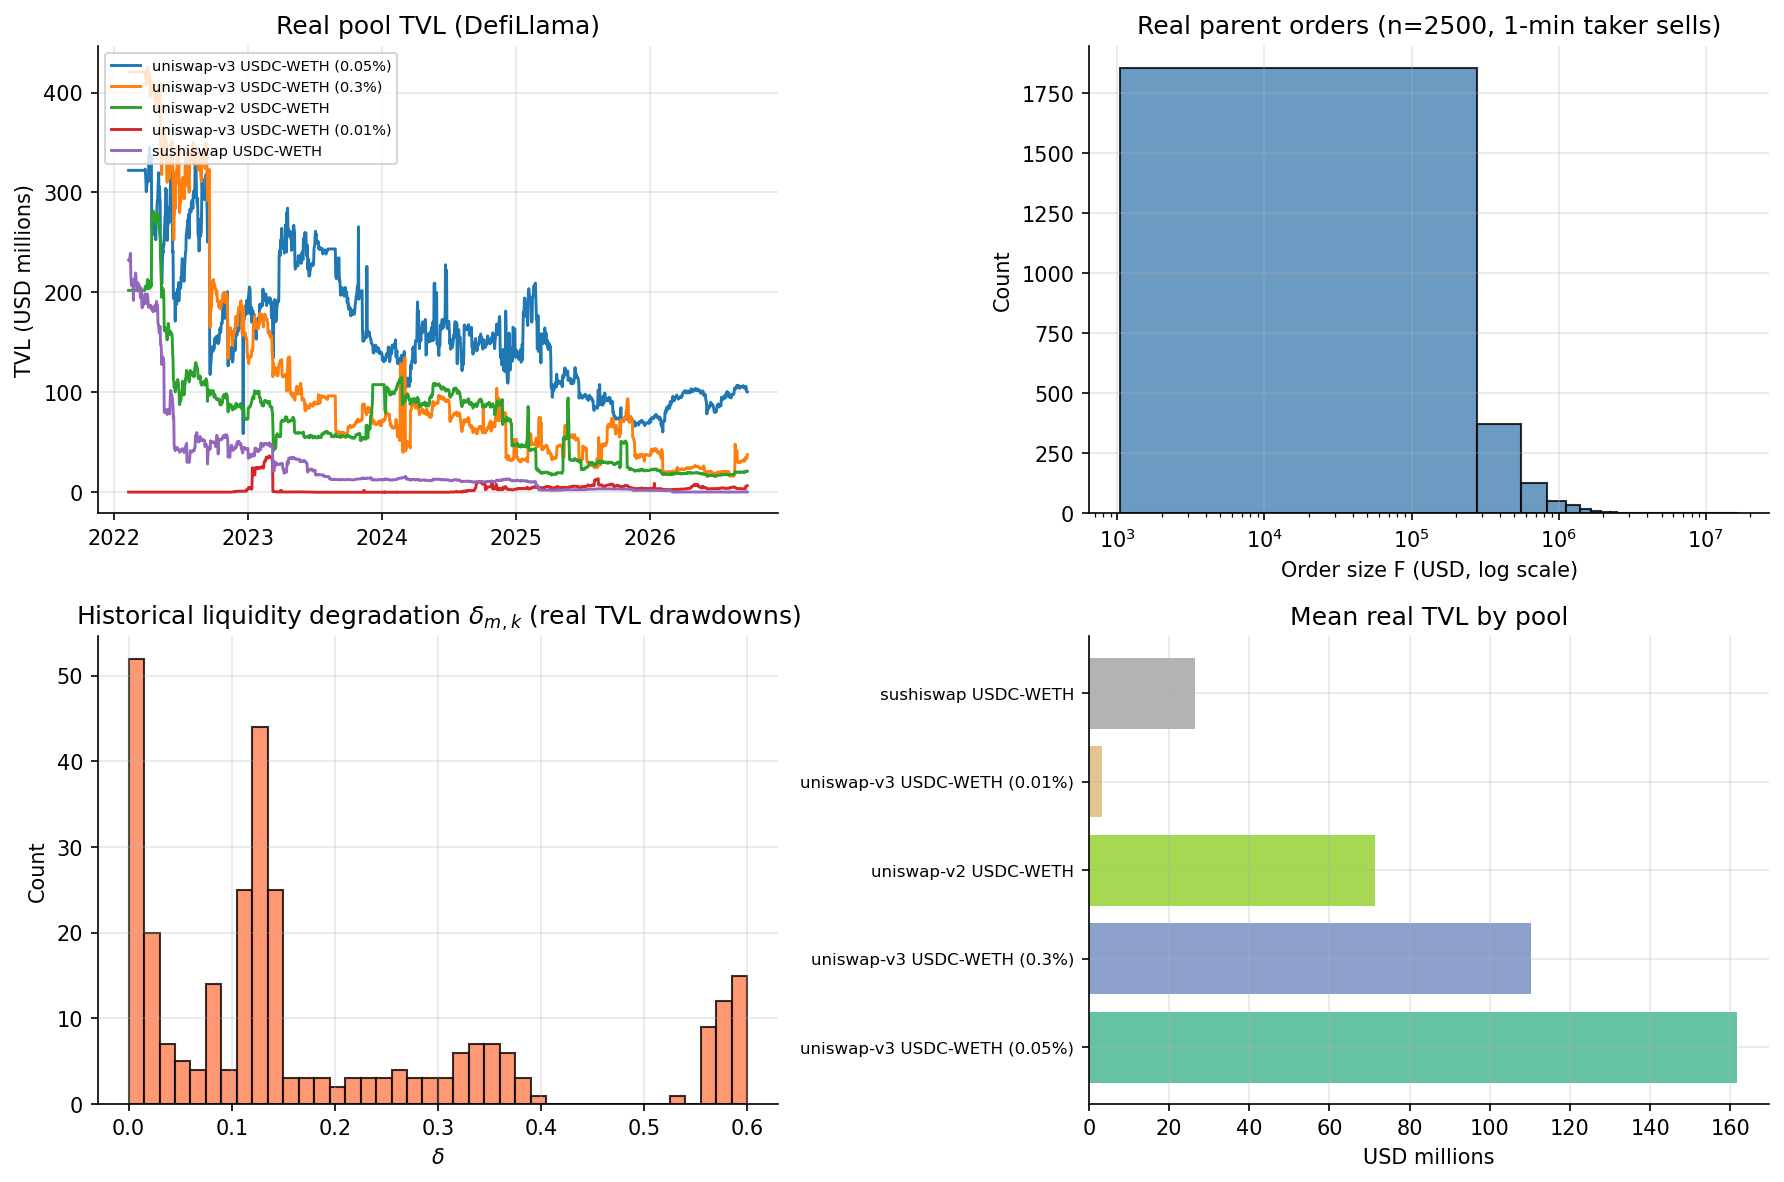
\includegraphics[width=0.98\linewidth]{01_data_overview.png}
\caption{Real data.  Top left: daily TVL of the five real pools (DefiLlama).  Top right:
size distribution of the 2{,}500 real parent orders (log scale).  Bottom left: empirical
distribution of the scenario liquidity deviations $\delta_{m,k}$ derived from real TVL.
Bottom right: mean real TVL by pool.}
\label{fig:data}
\end{figure}

% =====================================================================
\section{Convex cost model}
\label{sec:model}
% =====================================================================

\subsection{Exact cost of a constant-product trade}

A constant-product AMM holds reserves $(R_x,R_y)$ with invariant $R_xR_y=k$
\cite{adams2021uniswap,angeris2022optimal}.  Value both reserves in USD at the pre-trade
mid price $p$, and let $y$ denote the output-side reserve in USD.  Selling input notional
$n$ (USD) moves the trade along the curve; writing the input size in tokens as
$\mathrm{d}x = n/p$ and the output obtained as
$\mathrm{d}y = y\,\mathrm{d}x/(x+\mathrm{d}x)$, the price-impact cost versus the pre-trade
mid is

\begin{equation}
\label{eq:exact-cost}
  \text{cost}(n)\;=\; p\,\mathrm{d}x - \mathrm{d}y
  \;=\;\frac{n^{2}}{y+n}.
\end{equation}

For a balanced pool with total value $V$ we have $y = V/2$, and we define the
\emph{liquidity index}

\begin{equation}
\label{eq:L-def}
  L \;:=\; y \;=\; \frac{\mathrm{TVL}}{2}\qquad\text{(USD)}.
\end{equation}

The exact cost \eqref{eq:exact-cost} is convex in $n$ (it is the perspective-like function
$n\mapsto n^2/(y+n)$, whose second derivative $2y^2/(y+n)^3$ is positive).  Its second-order
Taylor expansion at $n=0$ is

\begin{equation}
\label{eq:taylor}
  \text{cost}(n) \;=\; \frac{n^{2}}{y} - \frac{n^{3}}{y^{2}} + \cdots
  \;=\; b\,\frac{n^{2}}{L} + O\!\left(\frac{n^{3}}{L^{2}}\right),
  \qquad b = 1,
\end{equation}

which is the quadratic surrogate prescribed by the project statement.  The relative error of
\eqref{eq:taylor} versus \eqref{eq:exact-cost} is 0.5\% at $0.1\%$ of the pool reserve, 1\%
at 1\% and 5\% at 5\% (verified numerically in the test suite).

\subsection{Fees and the full cost function}

AMM protocols charge the fee $\phi_m$ on the input token.  To first order this adds a linear
term, so the total cost of sending $f_m$ USD to pool $m$ with liquidity $L_m$ is

\begin{equation}
\label{eq:cost-m}
  c_m(f_m; L_m) \;=\; \underbrace{a_m f_m}_{\text{fee}}
  \;+\; \underbrace{b_m \frac{f_m^{2}}{L_m}}_{\text{price impact}},
  \qquad a_m = \phi_m,\quad b_m = 1,\quad f_m \ge 0.
\end{equation}

This is the form required by the statement ($a_m,b_m\ge 0$), it is convex (affine plus
quadratic-over-linear), and its parameters are pinned by real data: $\phi_m$ from the
protocol fee tiers (Table~\ref{tab:pools}) and $L_m$ from the real TVL.

\subsection{Fidelity check on the real trade tape}
\label{sec:tape}

Although \eqref{eq:cost-m} is derived for AMMs, its qualitative claim --- execution cost is
positive and increasing in order size --- can be checked on the real Binance tape, which also
anchors the linear fee/spread scale.  For every one-second window with aggressive sells we
compute the realised impact
$\text{cost} = (\text{pre-mid}-\text{vwap})/\text{pre-mid}\times n$ and fit
$\text{cost}\approx \hat a n + \hat b n^{2}$ to \emph{size-bin means} (binning averages out
bid/ask bounce):

\[
  \text{cost} \;\approx\; 1.28\cdot 10^{-4}\, n \;-\; 1.04\cdot 10^{-9}\, n^{2},
  \qquad R^{2} = 0.92,\quad 53{,}68 \text{ observations}.
\]

Cost is increasing in size (Spearman rank correlation 0.88) and rises from 0.54 to 0.71 bps
of notional between the smallest and largest bins.  The fitted \emph{linear} coefficient
(\,$\approx 1.3$ bps\,) is the fee-plus-spread scale we expect on a CEX.  The fitted
quadratic coefficient is small and negative: curvature on a central-limit-order book is
genuinely different from the constant-product curvature of \eqref{eq:exact-cost} (books
offer level liquidity and are resilient within a second).  The quadratic-in-$n$ impact used
throughout this report is therefore justified analytically by \eqref{eq:taylor} for AMM
pools; the tape confirms the positive, size-increasing structure and the linear scale.
Figure~\ref{fig:impact} shows the bin means and the fit.

\begin{figure}[H]
\centering
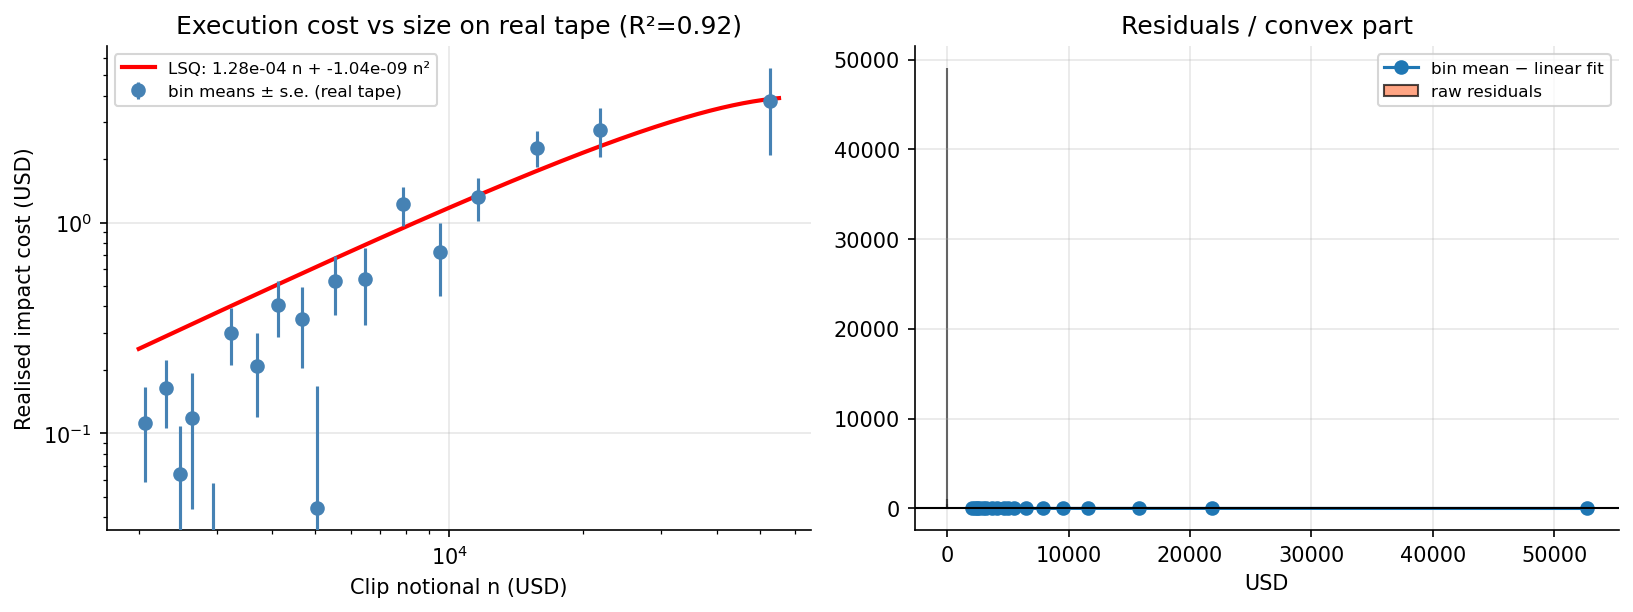
\includegraphics[width=0.92\linewidth]{02_impact_fidelity.png}
\caption{Execution cost on the real trade tape.  Left: size-bin means of one-second realised
impact (with standard errors) and the least-squares fit $\hat a n + \hat b n^{2}$.
Right: residuals and the convex part after removing the linear fit.}
\label{fig:impact}
\end{figure}

% =====================================================================
\section{Scenario model: uncertain execution quality}
\label{sec:scenarios}
% =====================================================================

The statement requires scenario liquidity degradations
\begin{equation}
\label{eq:scenario}
  L_{m,k} \;=\; L_m\,(1-\delta_{m,k}),\qquad \delta_{m,k}\in[0,\bar\delta),\quad \bar\delta=0.6,
\end{equation}
for $k=1,\dots,K$ adverse scenarios.  We build $\delta_{m,k}$ by \textbf{adverse historical
resampling of the real TVL series}.  Let $L_m(t)=\mathrm{TVL}_m(t)/2$ be the daily real
liquidity index and let $G_m$ be its geometric mean over the trailing 365 days (the pool's
\emph{typical level}).  For the decision day $d$,

\begin{equation}
\label{eq:delta}
  \delta_{m,k} \;=\; \min\!\Big(\big(1 - L_m(d-k)/G_m\big)_+,\; \bar\delta\Big),
  \qquad k=1,\dots,365,
\end{equation}

where $(\cdot)_+$ clips to the adverse side (the statement only admits degradation).
The scenario set keeps $K=120$ of those days: the 24 worst shortfall days (by mean
deviation across pools) plus a seeded uniform sample of the remainder.  The same historical
day is used for every pool, so cross-pool correlation (a market-wide liquidity event hits
all pools together) is preserved.  Only days strictly before the execution day enter
\eqref{eq:delta} (no look-ahead).

\begin{remark}[Why deviations are taken against $G_m$, not against ``today'']
A raw shortfall $1 - L_m(d-k)/L_m(d-1)$ confounds \emph{trend} with \emph{risk}: a pool that
has secularly grown looks permanently risky (its past sits below today) while a pool that
has \emph{collapsed} looks permanently safe (its past sits above today).  On the real data
this inversion is not academic --- it made the crashed SushiSwap pool look like the safest
one and the healthy Uniswap V3 0.05\% pool like the riskiest, tilting the optimal allocation
the wrong way.  Measuring shortfalls against the pool's own typical level $G_m$ restores the
correct ordering (Table~\ref{tab:pools}) and is covered by a regression test.
\end{remark}

At the reference date 2026-08-31 the sampled deviations have mean 0.163, median 0.103,
95th percentile 0.600 (the cap binds for the stressed pool) and maximum 0.600.

% =====================================================================
\section{Optimization problem}
\label{sec:problem}
% =====================================================================

\textbf{Decision variables}
\begin{align*}
  f_m &\ge 0 &&\text{USD sent to pool } m, \qquad \textstyle\sum_{m=1}^{M} f_m = F,\\
  z_m &\in[0,1] &&\text{usage variable of pool } m,\qquad f_m \le F z_m .
\end{align*}

\textbf{Scenario cost.}  With gas charged through the usage variables,
\begin{equation}
\label{eq:Ck}
  C_k(f) \;=\; \sum_{m=1}^{M}\Big(a_m f_m + b_m \frac{f_m^{2}}{L_{m,k}}\Big)
  \;+\; \sum_{m=1}^{M} g_m z_m .
\end{equation}

\textbf{Risk measure.}  For a level $\alpha\in(0,1)$ the Rockafellar--Uryasev
reformulation \cite{rockafellar2000optimization} of \cvar{} over the $K$ equiprobable
scenarios is
\begin{equation}
\label{eq:cvar}
  \cvar_\alpha(C) \;=\; \min_{t\in\mathbb{R},\, u\ge 0}
  \; t + \frac{1}{(1-\alpha)K}\sum_{k=1}^{K} u_k
  \qquad\text{s.t.}\qquad u_k \ge C_k(f) - t .
\end{equation}
The minimizing $t$ is a value-at-risk threshold, $\var_\alpha(C)=t^\star$.

\textbf{Problem.}  As in the project statement,
\begin{equation}
\label{eq:problem}
  \min_{f,z,t,u}\;
  \underbrace{\frac{1}{K}\sum_{k=1}^{K} C_k(f)}_{\text{expected cost}}
  \;+\; \lambda\, \cvar_\alpha(C)
  \;+\; \eta \sum_{m=1}^{M} z_m
\end{equation}
subject to $\sum_m f_m = F$, $f_m\ge 0$, $0\le z_m\le 1$, $f_m\le F z_m$, and the epigraph
constraints of \eqref{eq:cvar}.  The parameter $\lambda\ge 0$ trades expected cost against
tail cost, and $\eta\ge 0$ is the intended per-pool sparsity penalty.

\begin{remark}[Naming]
The statement writes $\var_\alpha$ for expression \eqref{eq:cvar}; that expression is
\cvar{} (mean excess loss / expected shortfall) and its optimal threshold is $\var_\alpha$.
We report both.
\end{remark}

% =====================================================================
\section{Convexity and DCP analysis}
\label{sec:convexity}
% =====================================================================

\begin{proposition}[Convexity of the scenario costs]
For every scenario $k$, the function $C_k$ in \eqref{eq:Ck} is convex on
$\{f\ge 0,\; 0\le z\le 1\}$.
\end{proposition}

\begin{proof}
The term $a_m f_m$ is affine.  The term $b_m f_m^{2}/L_{m,k}$ is the \emph{quadratic
over linear} function $\mathrm{qol}(f_m, L_{m,k}) = b_m f_m^2/L_{m,k}$ with $L_{m,k}>0$
constant; $\mathrm{qol}(x,y)=x^{2}/y$ is convex on $y>0$ (it is the perspective of
$x\mapsto x^{2}$, and its Hessian
$\frac{2}{y^{3}}\left(\begin{smallmatrix} y^{2} & -xy\\ -xy & x^{2}\end{smallmatrix}\right)$ is positive
semidefinite) \cite{boyd2004convex}.  The gas term $g_m z_m$ is affine in $z$.  Sums of
convex functions are convex.
\end{proof}

\begin{proposition}[Convexity of the full problem]
Problem \eqref{eq:problem} with the epigraph constraints of \eqref{eq:cvar} is a convex
program (a cone program with quadratic and linear pieces).
\end{proposition}

\begin{proof}
Substituting the epigraph variables, the objective
$\frac{1}{K}\sum_k C_k(f) + \lambda\big(t + \frac{1}{(1-\alpha)K}\sum_k u_k\big)
+ \eta\sum_m z_m$ is convex (Proposition~1 plus affine terms, weighted with non-negative
coefficients $\lambda\ge0$, $\eta\ge0$).  The constraints $u_k \ge C_k(f)-t$ are
sublevel-set constraints of the convex function $C_k(f)-t-u_k$ (equivalently: the epigraph
of a convex function is a convex set, shifted by affine terms), and all remaining
constraints are linear.  Hence the feasible set is convex and we minimize a convex function
over it.  In particular a local optimum is global.
\end{proof}

\subsection*{DCP mapping}

CVXPY verifies these curvature rules automatically (DCP).  Two equivalent DCP forms of the
impact term are used in the codebase:

\[
  \underbrace{\sum_{m} b_m\,
  \texttt{quad\_over\_lin}(f_m, L_{m,k})}_{\text{literal statement hint}}
  \qquad\equiv\qquad
  \underbrace{\big\|\mathrm{diag}\big(\sqrt{b/L_{k}}\big)\,f\big\|_{2}^{2}}_{\texttt{sum\_squares(multiply(w,f))}} .
\]

The left form is kept as a reference implementation and is cross-checked numerically against
the right form, which builds one atom per scenario instead of one per pool $\times$ scenario
(a large compile-time saving at $K\sim10^{2}$).  The full problem is additionally
\emph{DPP-compliant} (disciplined parametrized programming), which we exploit to compile it
once per $(M,K,\alpha,\lambda)$ and re-solve it through parameters for every order size and
every historical scenario set.

\subsection{The $z_m$ relaxation is fractional --- and collapses}
\label{sec:relaxation}

The statement replaces the binary indicator ``pool $m$ is used'' by
$0\le z_m\le 1$, $f_m\le F z_m$, penalized by $\eta\sum_m z_m$ (and, inside $C_k$, by
$g_m z_m$).  The intended effect is a fixed cost per pool used.  The following shows what
the relaxation actually does.

\begin{lemma}[Collapse of the usage variables]
\label{lem:collapse}
If $g_m+\eta>0$ for pool $m$, then every optimal solution of \eqref{eq:problem} satisfies
$z_m = f_m/F$.  Consequently $\sum_m z_m = 1$ at every feasible point with $\sum_m f_m=F$
that is optimal, so the sparsity penalty $\eta\sum_m z_m$ is the constant $\eta$ and has no
influence on the allocation.
\end{lemma}

\begin{proof}
The objective is non-decreasing in each $z_m$ (with positive coefficient $g_m+\eta$ on the
scenarios and $\eta$), while the only constraint coupling $z_m$ from below is
$z_m \ge f_m/F$ (together with $z_m\le 1$, which is never binding at the lower bound since
$f_m\le F$).  Hence $z_m$ is driven to its lower bound $f_m/F$.  Summing over $m$ gives
$\sum_m z_m = \sum_m f_m/F = 1$.
\end{proof}

\begin{remark}[Consequences]
Lemma~\ref{lem:collapse} makes the gas term of \eqref{eq:Ck} \emph{proportional},
$\sum_m g_m f_m/F$, rather than a fixed charge $g_m\mathbf{1}\{f_m>0\}$.  For large orders
this is a good approximation (a \$10 clip really is dominated by the per-dollar term
$g_m/F$), but it \emph{underprices splitting for small orders}: the relaxed optimum splits
even when a second pool's gas exceeds the impact it saves.  This gap is measured in
Section~\ref{sec:sensitivity-F} and is one reason to evaluate every strategy under the
\emph{true} economic cost
\begin{equation}
\label{eq:true-cost}
  \text{true-cost}(f) \;=\; \sum_m a_m f_m + b_m \frac{f_m^{2}}{L_m}
  \;+\!\!\sum_{m:\,f_m>0}\!\! g_m ,
\end{equation}
which we do everywhere (baselines and backtest).  A cheap practical fix --- the
\emph{gas-guard} strategy of Section~\ref{sec:backtest} --- compares the relaxed solution
with the best single pool under \eqref{eq:true-cost} and keeps the cheaper.
\end{remark}

% =====================================================================
\section{Numerical solution in CVXPY}
\label{sec:numerics}
% =====================================================================

Problem \eqref{eq:problem} is implemented with \textbf{CVXPY} and solved with
\textbf{CLARABEL} (interior point), with SCS as an automatic fallback; every solve returns
status \code{optimal} in our experiments.  The base-case dimensions are

\begin{center}
\small
\begin{tabular}{@{}llllll@{}}
\toprule
$M$ & $K$ & variables $(f,z,t,u)$ & constraints & solver & warm solve time \\
\midrule
5 & 120 & $5+5+1+120 = 131$ & $251$ & CLARABEL & 14.6 ms \\
\bottomrule
\end{tabular}
\end{center}

\medskip
\noindent
(cold start including CVXPY compilation of the parametrized problem: 0.3--1 s at this size;
the compile is paid once per problem structure.)  A warm-up solve precedes all reported
timings.

\paragraph{Scalability.}
Table~\ref{tab:scaling} and Figure~\ref{fig:scaling} report solve time for random pool sets
in the real parameter ranges.  Warm re-solves scale gently (5.6 ms at $(M,K)=(5,50)$ to
66.5 ms at $(20,200)$) while cold compilation grows superlinearly in $K$.

\begin{table}[H]
\centering
\caption{Solver scalability: warm re-solve time vs.\ cold compile+solve time (ms).}
\label{tab:scaling}
\small
\begin{tabular}{@{}rrrrrr@{}}
\toprule
$M$ & $K$ & \textbf{warm (ms)} & \textbf{cold (ms)} & variables & constraints \\
\midrule
5 & 50  & 5.6  & 328   & 61  & 111 \\
5 & 100 & 10.8 & 631   & 111 & 211 \\
5 & 200 & 23.3 & 2{,}666 & 211 & 411 \\
10 & 50  & 8.6  & 338   & 71  & 121 \\
10 & 100 & 14.9 & 1{,}424 & 121 & 221 \\
10 & 200 & 38.5 & 10{,}028 & 221 & 421 \\
20 & 50  & 15.0 & 671   & 91  & 141 \\
20 & 100 & 28.6 & 4{,}041 & 141 & 241 \\
20 & 200 & 66.5 & 33{,}152 & 241 & 441 \\
\bottomrule
\end{tabular}
\end{table}

\begin{figure}[H]
\centering
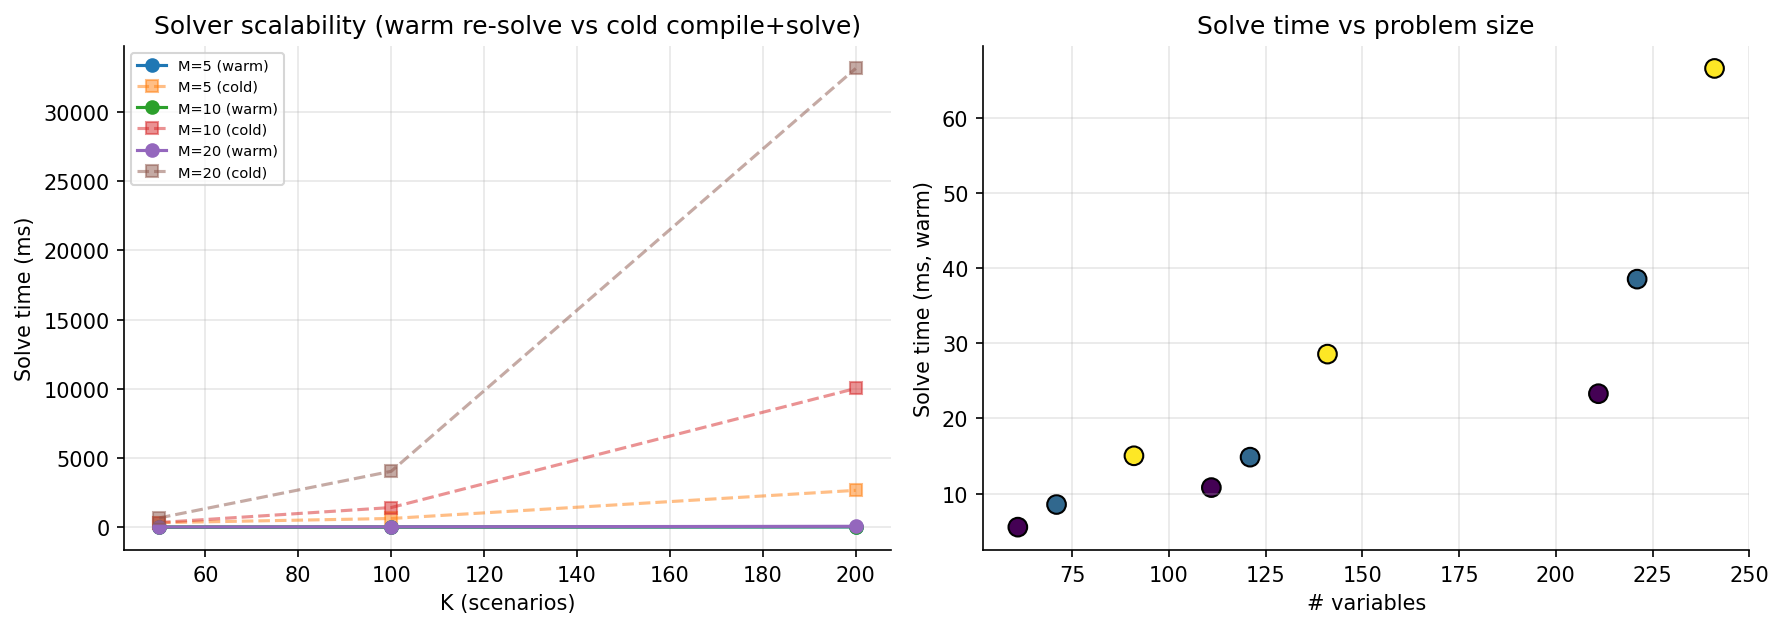
\includegraphics[width=0.92\linewidth]{09_scalability.png}
\caption{Solver scalability.  Left: warm re-solve (solid) vs.\ cold compile+solve (dashed)
against the number of scenarios $K$, per pool count $M$.  Right: warm solve time versus
problem size.}
\label{fig:scaling}
\end{figure}

% =====================================================================
\section{Base-case solution}
\label{sec:basecase}
% =====================================================================

Base-case parameters: order size $F=\$250{,}000$, $\alpha=0.95$, $\lambda=1$,
$\eta=0$ (Lemma~\ref{lem:collapse}), reference date 2026-08-31, $K=120$ scenarios from the
trailing year of real TVL deviations.

\begin{table}[H]
\centering
\caption{Optimal allocation of a \$250{,}000 order (\cvar{} router).}
\label{tab:basecase}
\small
\begin{tabular}{@{}lrrrr@{}}
\toprule
\textbf{Pool} & $f_m$ \textbf{(USD)} & \textbf{share} & $z_m$ & $\phi_m$ \\
\midrule
Uniswap V3 0.05\% & 184{,}531 & 73.8\% & 0.738 & 0.05\% \\
Uniswap V3 0.3\%  & 33{,}374  & 13.3\% & 0.133 & 0.30\% \\
Uniswap V2        & 25{,}712  & 10.3\% & 0.103 & 0.30\% \\
Uniswap V3 0.01\% & 6{,}104   &  2.4\% & 0.024 & 0.01\% \\
SushiSwap         & 278       &  0.1\% & 0.001 & 0.30\% \\
\midrule
\multicolumn{2}{@{}l}{optimal objective} & \multicolumn{3}{@{}r@{}}{\$2{,}436.76} \\
\multicolumn{2}{@{}l}{expected cost $\frac{1}{K}\sum_k C_k$} & \multicolumn{3}{@{}r@{}}{\$1{,}194.39} \\
\multicolumn{2}{@{}l}{$\cvar_{0.95}$ (true cost, scenario set)} & \multicolumn{3}{@{}r@{}}{\$1{,}308.86} \\
\multicolumn{2}{@{}l}{$\var_{0.95} = t^\star$} & \multicolumn{3}{@{}r@{}}{\$1{,}234.95} \\
\bottomrule
\end{tabular}
\end{table}

\begin{figure}[H]
\centering
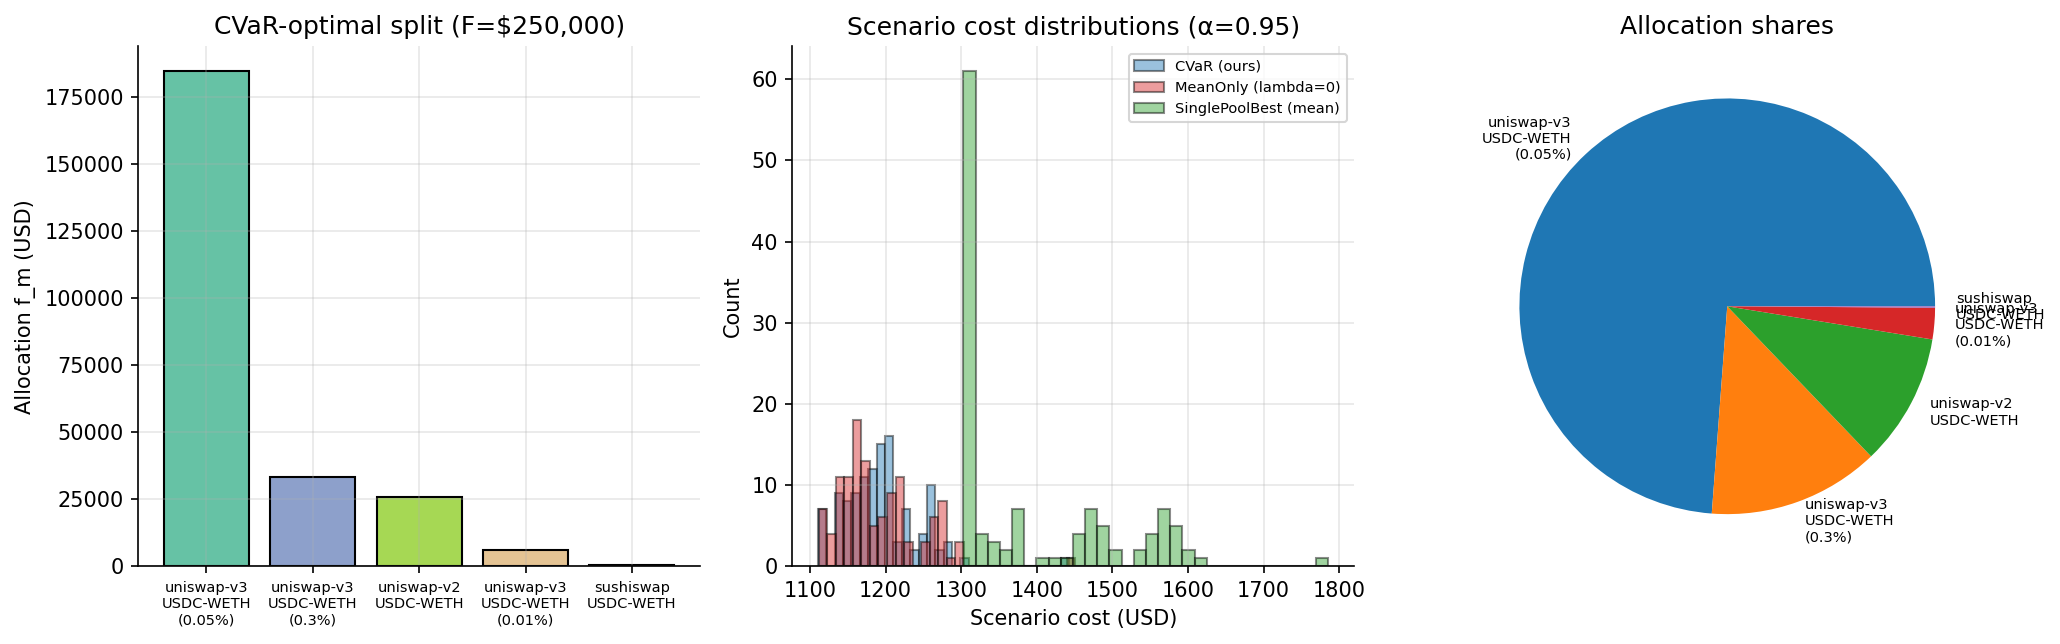
\includegraphics[width=0.98\linewidth]{03_base_case_allocation.png}
\caption{Base-case allocation of \$250{,}000 across the five real pools (left), the
resulting scenario-cost distributions of the competing strategies (middle), and the
allocation shares (right).}
\label{fig:basecase}
\end{figure}

The allocation concentrates on the deep, cheap 0.05\% tier (73.8\%) but spills into the
other tiers: impact is quadratic while fees are linear, so the last dollars are cheaper in
a second pool than in the first.  As $z_m=f_m/L$ collapses (Lemma~\ref{lem:collapse}) the
usage variables reproduce the allocation shares exactly.

% =====================================================================
\section{Baseline comparison}
\label{sec:baselines}
% =====================================================================

The statement requires two baselines: \textbf{(i) single-pool best} (the whole order in the
pool with the lowest mean cost, equivalently the deepest pool here) and \textbf{(ii)
mean-only} (the same problem with $\lambda=0$).  We add two labelled extras (equal split and
liquidity-proportional split) for context.  All strategies are evaluated with the true cost
\eqref{eq:true-cost} on the same 120-scenario set.

\begin{table}[H]
\centering
\caption{In-sample scenario costs by strategy (USD, true cost).}
\label{tab:baselines}
\small
\begin{tabular}{@{}lrrrrr@{}}
\toprule
\textbf{Strategy} & \textbf{mean} & $\var_{0.95}$ & $\cvar_{0.95}$ & \textbf{max} &
\textbf{\#pools} \\
\midrule
\cvar{} router (ours, $\lambda=1$) & 1{,}194.39 & \textbf{1{,}266.43} & \textbf{1{,}308.86} &
\textbf{1{,}442.99} & 4 \\
Mean-only ($\lambda=0$) & \textbf{1{,}191.32} & 1{,}278.21 & 1{,}317.94 & 1{,}450.71 & 4 \\
Single-pool best (mean cost) & 1{,}389.49 & 1{,}581.27 & 1{,}628.13 & 1{,}785.72 & 1 \\
Single-pool deepest (max $L_m$) & 1{,}389.49 & 1{,}581.27 & 1{,}628.13 & 1{,}785.72 & 1 \\
Equal split (extra) & 34{,}882.79 & 48{,}487.34 & 48{,}563.26 & 48{,}600.49 & 5 \\
Liquidity-proportional (extra) & 1{,}218.11 & 1{,}274.32 & 1{,}314.78 & 1{,}447.98 & 4 \\
\bottomrule
\end{tabular}
\end{table}

Relative to the best single pool the \cvar{} router cuts $\cvar_{0.95}$ by \textbf{19.6\%}
(\$319 per \$250k order); relative to mean-only it buys a 0.7\% tail reduction for 0.26\%
higher mean cost --- the expected trade-off shape of $\lambda\,\cvar_\alpha$ in
\eqref{eq:problem}.  Equal split is catastrophic (\$34.9k mean): putting \$50k into the
\$0.14M-liquidity SushiSwap pool costs more in impact than the entire order costs
optimally, which is exactly the quadratic term of \eqref{eq:cost-m} at work.

\begin{figure}[H]
\centering
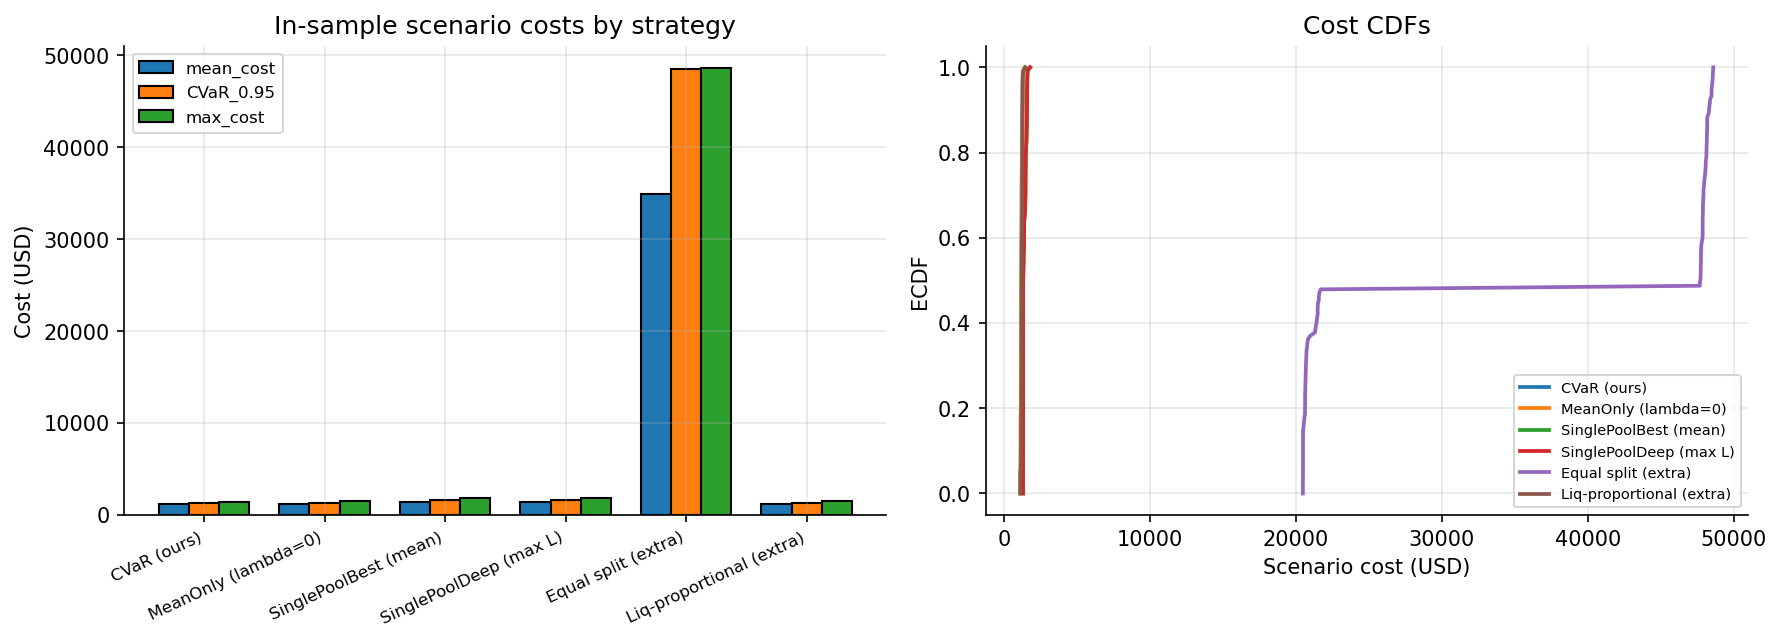
\includegraphics[width=0.98\linewidth]{04_baselines_insample.png}
\caption{Baseline comparison on the scenario set.  Left: mean, $\cvar_{0.95}$ and worst-case
cost per strategy.  Right: empirical cost distributions.}
\label{fig:baselines}
\end{figure}

% =====================================================================
\section{Sensitivity analysis}
\label{sec:sensitivity}
% =====================================================================

\subsection{Confidence level $\alpha$ (risk aversion)}
\label{sec:sensitivity-alpha}

\begin{table}[H]
\centering
\caption{Sweep over $\alpha$ at $F=\$250$k, $\lambda=1$.  $\cvar$(eval) is always measured
at the fixed level 0.95 for comparability; $\cvar$(own $\alpha$) is measured at the
solver's own level.}
\label{tab:sens-alpha}
\small
\begin{tabular}{@{}rrrrrrr@{}}
\toprule
$\alpha$ & \textbf{mean} & $\cvar$(eval, 0.95) & $\cvar$(own $\alpha$) & $\var_{0.95}$ &
\textbf{max} & \textbf{active pools} \\
\midrule
0.80 & 1{,}194.30 & 1{,}309.13 & 1{,}267.54 & 1{,}266.28 & 1{,}443.88 & 4 \\
0.90 & 1{,}195.20 & 1{,}308.24 & 1{,}285.12 & 1{,}265.07 & 1{,}443.13 & 4 \\
0.95 & 1{,}194.39 & 1{,}308.86 & 1{,}308.86 & 1{,}266.43 & 1{,}442.99 & 4 \\
0.99 & 1{,}193.39 & 1{,}310.98 & 1{,}418.81 & 1{,}270.17 & 1{,}443.18 & 4 \\
\bottomrule
\end{tabular}
\end{table}

\begin{figure}[H]
\centering
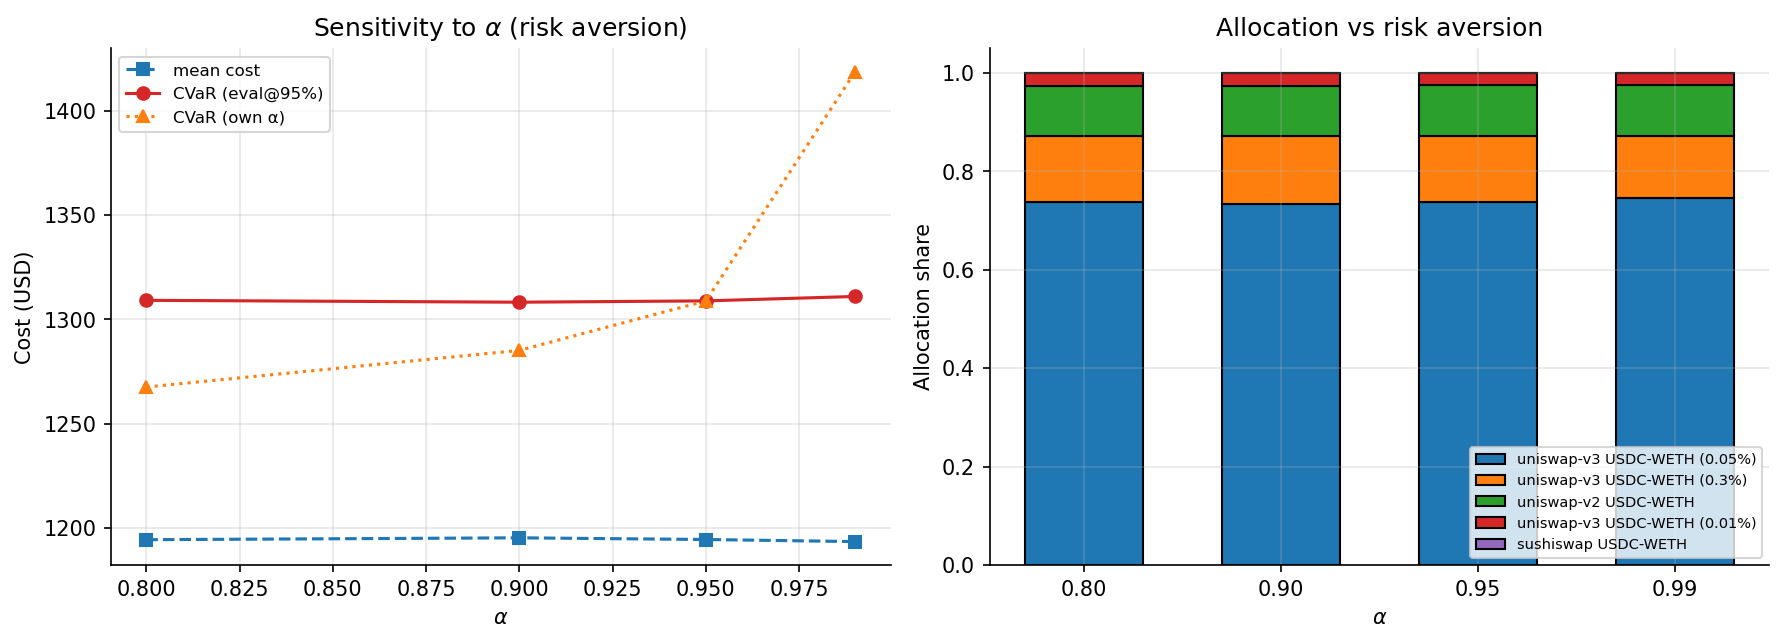
\includegraphics[width=0.92\linewidth]{05_sensitivity_alpha.png}
\caption{Sensitivity to $\alpha$.  Left: mean cost (flat) and \cvar{} at the solver's own
level (rising with $\alpha$, since a deeper tail is averaged).  Right: allocation shares
shift only mildly toward the low-deviation 0.05\% tier as risk aversion grows.}
\label{fig:sens-alpha}
\end{figure}

Risk-averse settings shift a little weight from the high-deviation Uniswap V3 0.3\% tier
($\bar\delta=0.21$) toward the low-deviation 0.05\% tier ($\bar\delta=0.06$).  Costs measured
at a \emph{fixed} evaluation level stay flat because the five real pools have similar tail
costs at this order size; the \cvar{} measured at the solver's own level grows from
\$1{,}268 to \$1{,}419 as $\alpha$ goes from 0.80 to 0.99 simply because a deeper tail
(1\% instead of 20\%) is being averaged.

\subsection{Order size $F$: when does splitting become necessary?}
\label{sec:sensitivity-F}

\begin{table}[H]
\centering
\caption{Sweep over the order size $F$ (true cost).  \cvar{} router vs.\ the best single
pool; ``active pools'' counts pools with more than 1\% of $F$.}
\label{tab:sens-F}
\small
\begin{tabular}{@{}rrrrrr@{}}
\toprule
$F$ \textbf{(USD)} & \textbf{active pools} & \textbf{router mean} & \textbf{router $\cvar_{0.95}$} &
\textbf{single-pool mean} & \textbf{router bps of } $F$ \\
\midrule
1{,}000    & 2 & 18.71 & 18.73 & \textbf{9.65} & 187.1 \\
5{,}000    & 2 & 21.13 & 21.22 & \textbf{12.13} & 42.3 \\
10{,}000   & 2 & 25.03 & 25.39 & \textbf{16.14} & 25.0 \\
50{,}000   & 2 & 91.33 & 100.31 & \textbf{84.35} & 18.3 \\
100{,}000  & 4 & 279.44 & 305.58 & \textbf{259.99} & 27.9 \\
500{,}000  & 4 & \textbf{4{,}111.99} & \textbf{4{,}520.94} & 5{,}280.57 & 82.2 \\
1{,}000{,}000 & 4 & \textbf{15{,}186.25} & \textbf{16{,}741.62} & 20{,}594.90 & 151.9 \\
5{,}000{,}000 & 4 & \textbf{354{,}731} & \textbf{393{,}344} & 504{,}653 & 709.5 \\
\bottomrule
\end{tabular}
\end{table}

\begin{figure}[H]
\centering
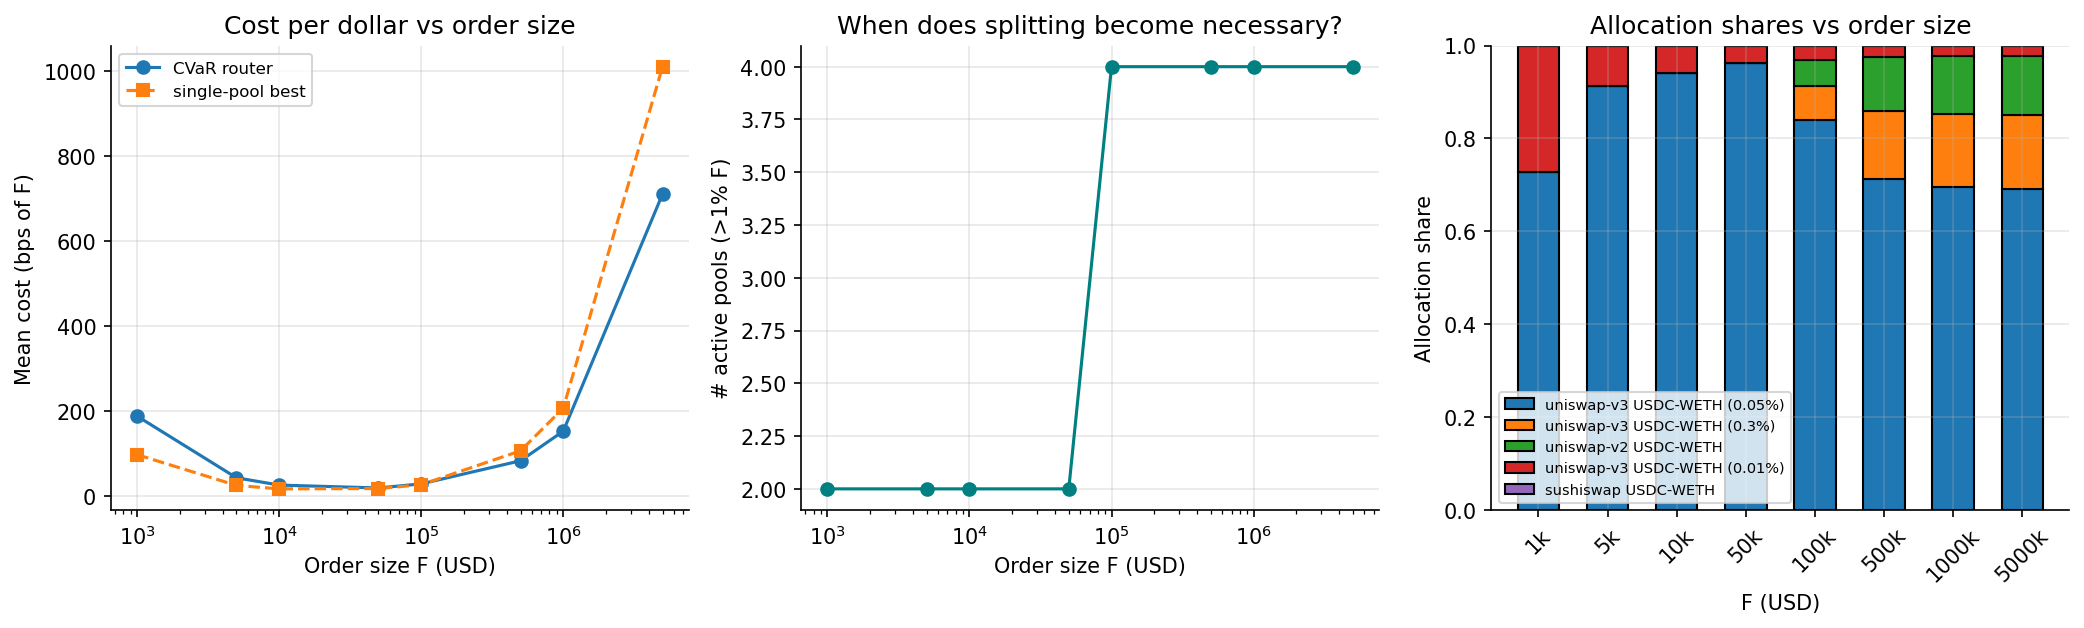
\includegraphics[width=0.98\linewidth]{06_sensitivity_size.png}
\caption{Sensitivity to the order size.  Left: cost per dollar (U-shaped: gas-dominated
small orders, impact-dominated large orders).  Middle: number of active pools --- splitting
starts paying around $F\approx \$100$--$200$k under true gas.  Right: allocation shares.}
\label{fig:sens-F}
\end{figure}

\textbf{Splitting becomes necessary at $F\approx \$100$--$200$k.}  Below that threshold the
relaxed model already splits in two pools but under the true fixed-gas cost
\eqref{eq:true-cost} the best single pool is cheaper (this is the relaxation gap of
Lemma~\ref{lem:collapse} made visible).  Above the threshold impact dominates and splitting
wins increasingly: $-22\%$ mean cost at $F=\$500$k and $-30\%$ at $F=\$5$M relative to the
best single pool.  Cost per dollar is U-shaped overall.

\subsection{Uncertainty intensity $\delta$: how much does \cvar{} protect the plan?}
\label{sec:sensitivity-delta}

Scaling the deviations in \eqref{eq:delta} by $s\in\{0,0.5,1,1.5,2\}$ (capped at
$\bar\delta$) interpolates between a certain world and twice the historically observed
liquidity stress.

\begin{table}[H]
\centering
\caption{Sweep over the uncertainty intensity.  Scenario-set costs of the \cvar{} plan
($\lambda=1$) and of the mean-only plan ($\lambda=0$), both evaluated at $\cvar_{0.95}$.}
\label{tab:sens-delta}
\small
\begin{tabular}{@{}rlrrrr@{}}
\toprule
\textbf{scale} & \textbf{plan} & \textbf{mean} & $\cvar_{0.95}$ & $\var_{0.95}$ &
\textbf{max} \\
\midrule
0.0 & \cvar{}     & 1{,}109.24 & 1{,}109.24 & 1{,}109.24 & 1{,}109.24 \\
0.0 & mean-only & 1{,}109.24 & 1{,}109.24 & 1{,}109.24 & 1{,}109.24 \\
\midrule
0.5 & \cvar{}     & 1{,}145.97 & 1{,}196.43 & 1{,}179.88 & 1{,}247.50 \\
0.5 & mean-only & 1{,}145.36 & 1{,}198.21 & 1{,}182.23 & 1{,}248.87 \\
\midrule
1.0 & \cvar{}     & 1{,}194.39 & 1{,}308.86 & 1{,}266.43 & 1{,}442.99 \\
1.0 & mean-only & 1{,}191.32 & 1{,}317.94 & 1{,}278.21 & 1{,}450.71 \\
\midrule
1.5 & \cvar{}     & 1{,}263.62 & 1{,}471.94 & 1{,}372.69 & 1{,}742.13 \\
1.5 & mean-only & 1{,}251.07 & 1{,}508.66 & 1{,}409.70 & 1{,}763.64 \\
\midrule
2.0 & \cvar{}     & 1{,}313.69 & 1{,}629.26 & 1{,}499.48 & \textbf{2{,}156.44} \\
2.0 & mean-only & 1{,}295.30 & 1{,}688.71 & 1{,}561.44 & 2{,}235.95 \\
\bottomrule
\end{tabular}
\end{table}

\begin{figure}[H]
\centering
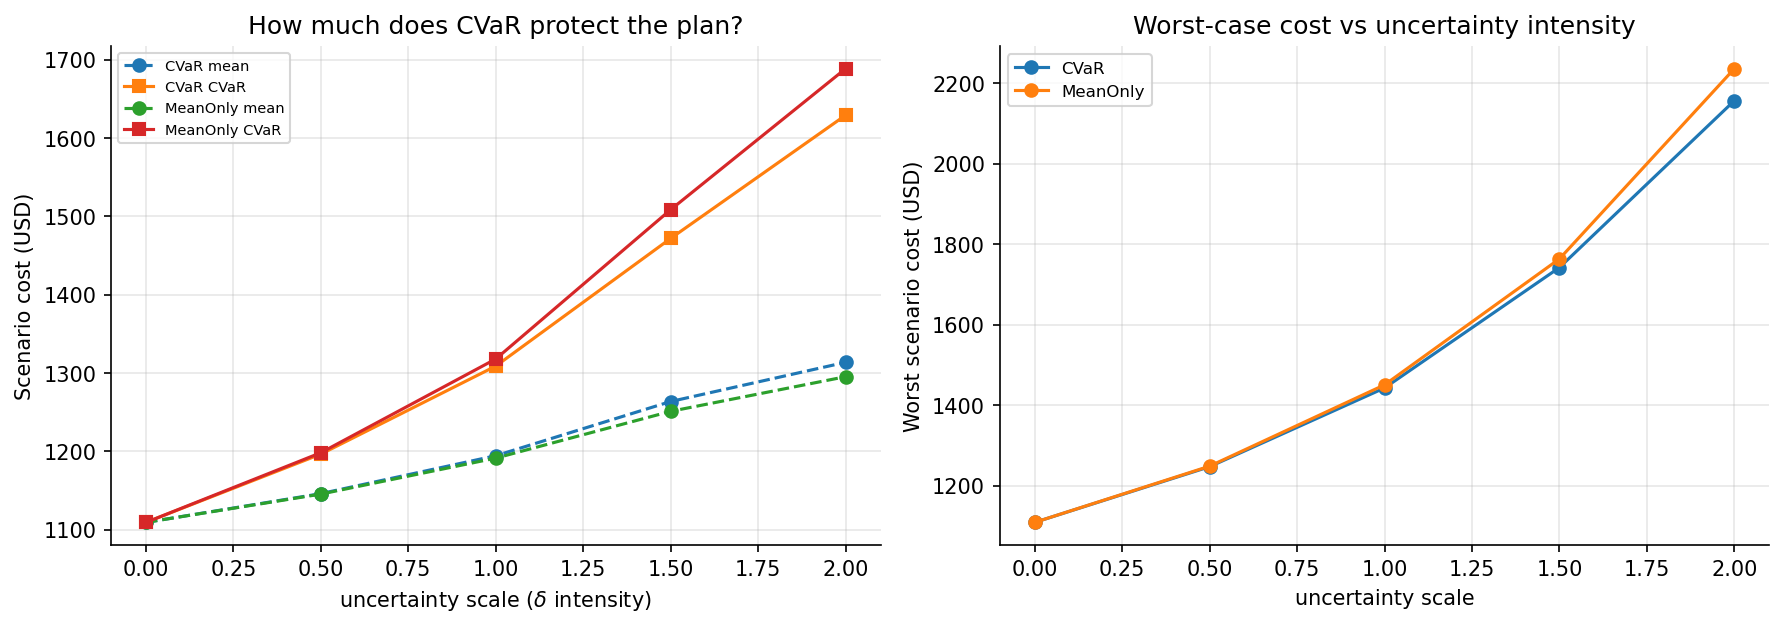
\includegraphics[width=0.92\linewidth]{07_sensitivity_delta.png}
\caption{Sensitivity to the uncertainty intensity.  As stress grows, the \cvar{} plan gives
up a little mean cost (1.4\% at scale 2.0) and its tail cost improves relative to the
mean-only plan (3.5\% at scale 2.0) --- the insurance premium of \cvar{} is small in calm
conditions and pays exactly when liquidity uncertainty is high.}
\label{fig:sens-delta}
\end{figure}

\subsection{Extra: efficient frontier in $\lambda$}

Varying $\lambda$ traces the supported Pareto set between expected and tail cost: over
$\lambda=0\to 8$ the mean rises from \$1{,}191 to \$1{,}201 while $\cvar_{0.95}$ falls from
\$1{,}318 to \$1{,}306.  The frontier is shallow (the five pools have correlated risk
factors) but strictly ordered.

\begin{figure}[H]
\centering
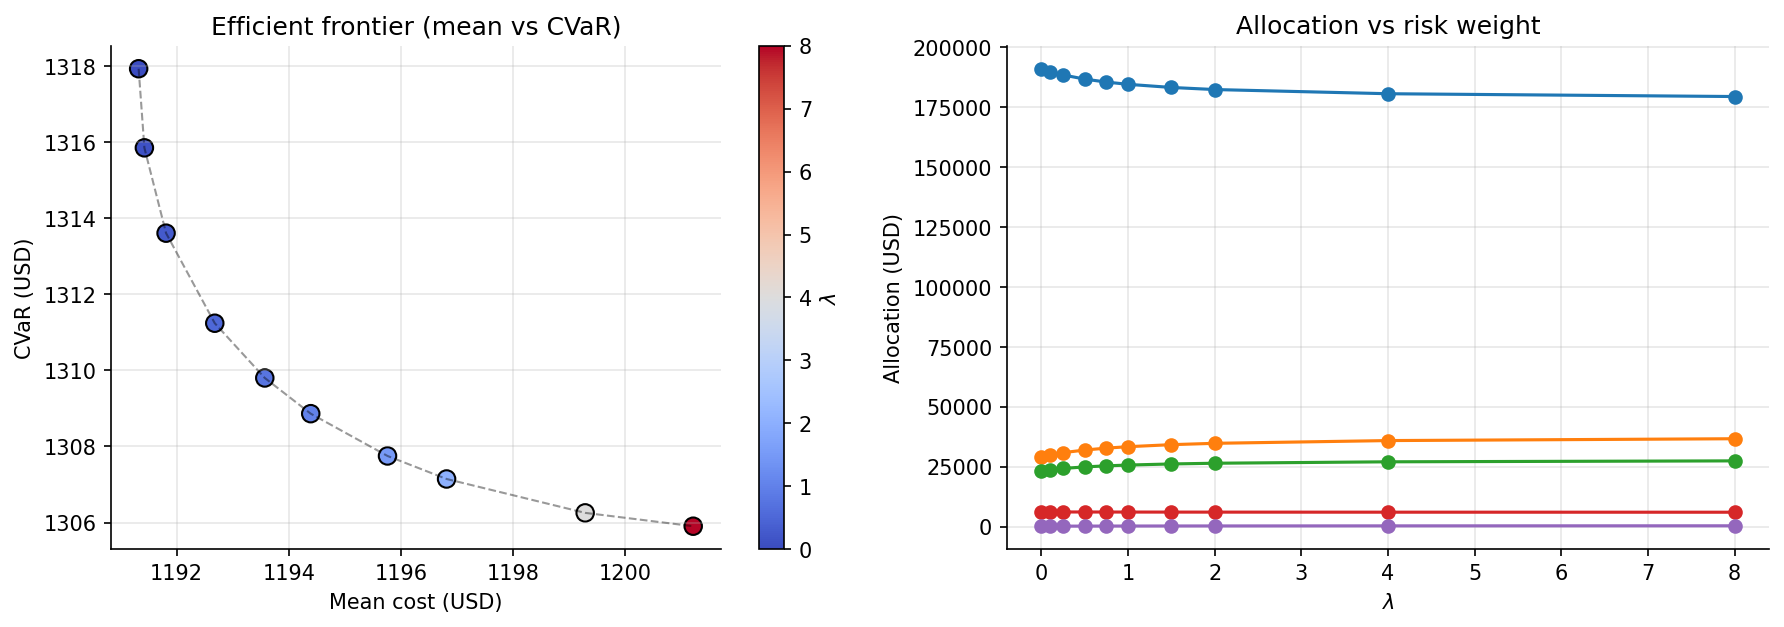
\includegraphics[width=0.92\linewidth]{08_frontier.png}
\caption{Efficient frontier (mean vs.\ \cvar) and the evolution of the allocation with the
risk weight $\lambda$.}
\label{fig:frontier}
\end{figure}

% =====================================================================
\section{Walk-forward backtest on real trades}
\label{sec:backtest}
% =====================================================================

The question the in-sample tables cannot answer is whether the router is still better when
the liquidity state that actually occurs was \emph{unknown} at decision time.  We therefore
run a walk-forward backtest over the 2{,}500 real parent orders of Section~\ref{sec:data}.

\begin{algorithm}[H]
\caption{Walk-forward backtest (per real parent order).}
\label{alg:backtest}
\begin{algorithmic}[1]
\Require order with real timestamp $t$ and real size $F$ (USD); real TVL histories
\State $\mathcal{S}(t) \gets$ scenario set from TVL strictly before day($t$)
        \Comment{no look-ahead}
\State $L^{\text{real}} \gets$ actual pool liquidity on day($t$) \Comment{out of sample}
\State $f^{\cvar} \gets$ solve \eqref{eq:problem} with $\lambda=1$ for size $F$ on
        $\mathcal{S}(t)$
\State $f^{\text{mean}} \gets$ solve \eqref{eq:problem} with $\lambda=0$ (mean-only)
\State $f^{\text{sp}} \gets$ best single pool (mean cost on $\mathcal{S}(t)$);
        $f^{\text{deep}} \gets$ deepest pool; $f^{\text{eq}}$, $f^{\text{prop}}$ extras
\State \textbf{gas-guard:} $f^{\text{guard}} \gets$ the cheaper of $f^{\cvar}$ and
        $f^{\text{sp}}$ under \eqref{eq:true-cost} on $\mathcal{S}(t)$
\For{each strategy $f$}
  \State record realized cost $\text{true-cost}(f;\, L^{\text{real}})$ \eqref{eq:true-cost}
\EndFor
\end{algorithmic}
\end{algorithm}

Realized costs are then aggregated into means, $\var_{0.95}$, $\cvar_{0.95}$ (the same
expected-shortfall estimator as in \eqref{eq:cvar}) and paired per-order comparisons.

\subsection{Realised costs over 2{,}500 real orders}

\begin{table}[H]
\centering
\caption{Realized execution costs on the real trade tape (2{,}500 orders, USD and bps of
$F$).}
\label{tab:backtest}
\small
\begin{tabular}{@{}lrrrrrr@{}}
\toprule
\textbf{Strategy} & \textbf{mean} & \textbf{median} & $\var_{0.95}$ & $\cvar_{0.95}$ &
\textbf{max} & \textbf{mean bps} \\
\midrule
\cvar{} + gas-guard & \textbf{6{,}902} & 414 & 12{,}178 & \textbf{117{,}000} & 3.47M &
\textbf{48.2} \\
\cvar{} router & 6{,}909 & 414 & 12{,}178 & 117{,}000 & 3.47M & 50.4 \\
Mean-only & 6{,}917 & \textbf{414} & 12{,}205 & 117{,}140 & 3.47M & 50.4 \\
Liquidity-prop.\ (extra) & 6{,}922 & 434 & 12{,}173 & 116{,}848 & 3.46M & 57.4 \\
Single-pool best & 9{,}987 & 422 & 17{,}037 & 172{,}781 & 5.25M & 60.3 \\
Single-pool deepest & 9{,}987 & 422 & 17{,}037 & 172{,}781 & 5.25M & 60.3 \\
Equal split (extra) & 166{,}132 & 6{,}162 & 280{,}810 & 2{,}895{,}020 & 88.3M & 922.6 \\
\bottomrule
\end{tabular}
\end{table}

\begin{figure}[H]
\centering
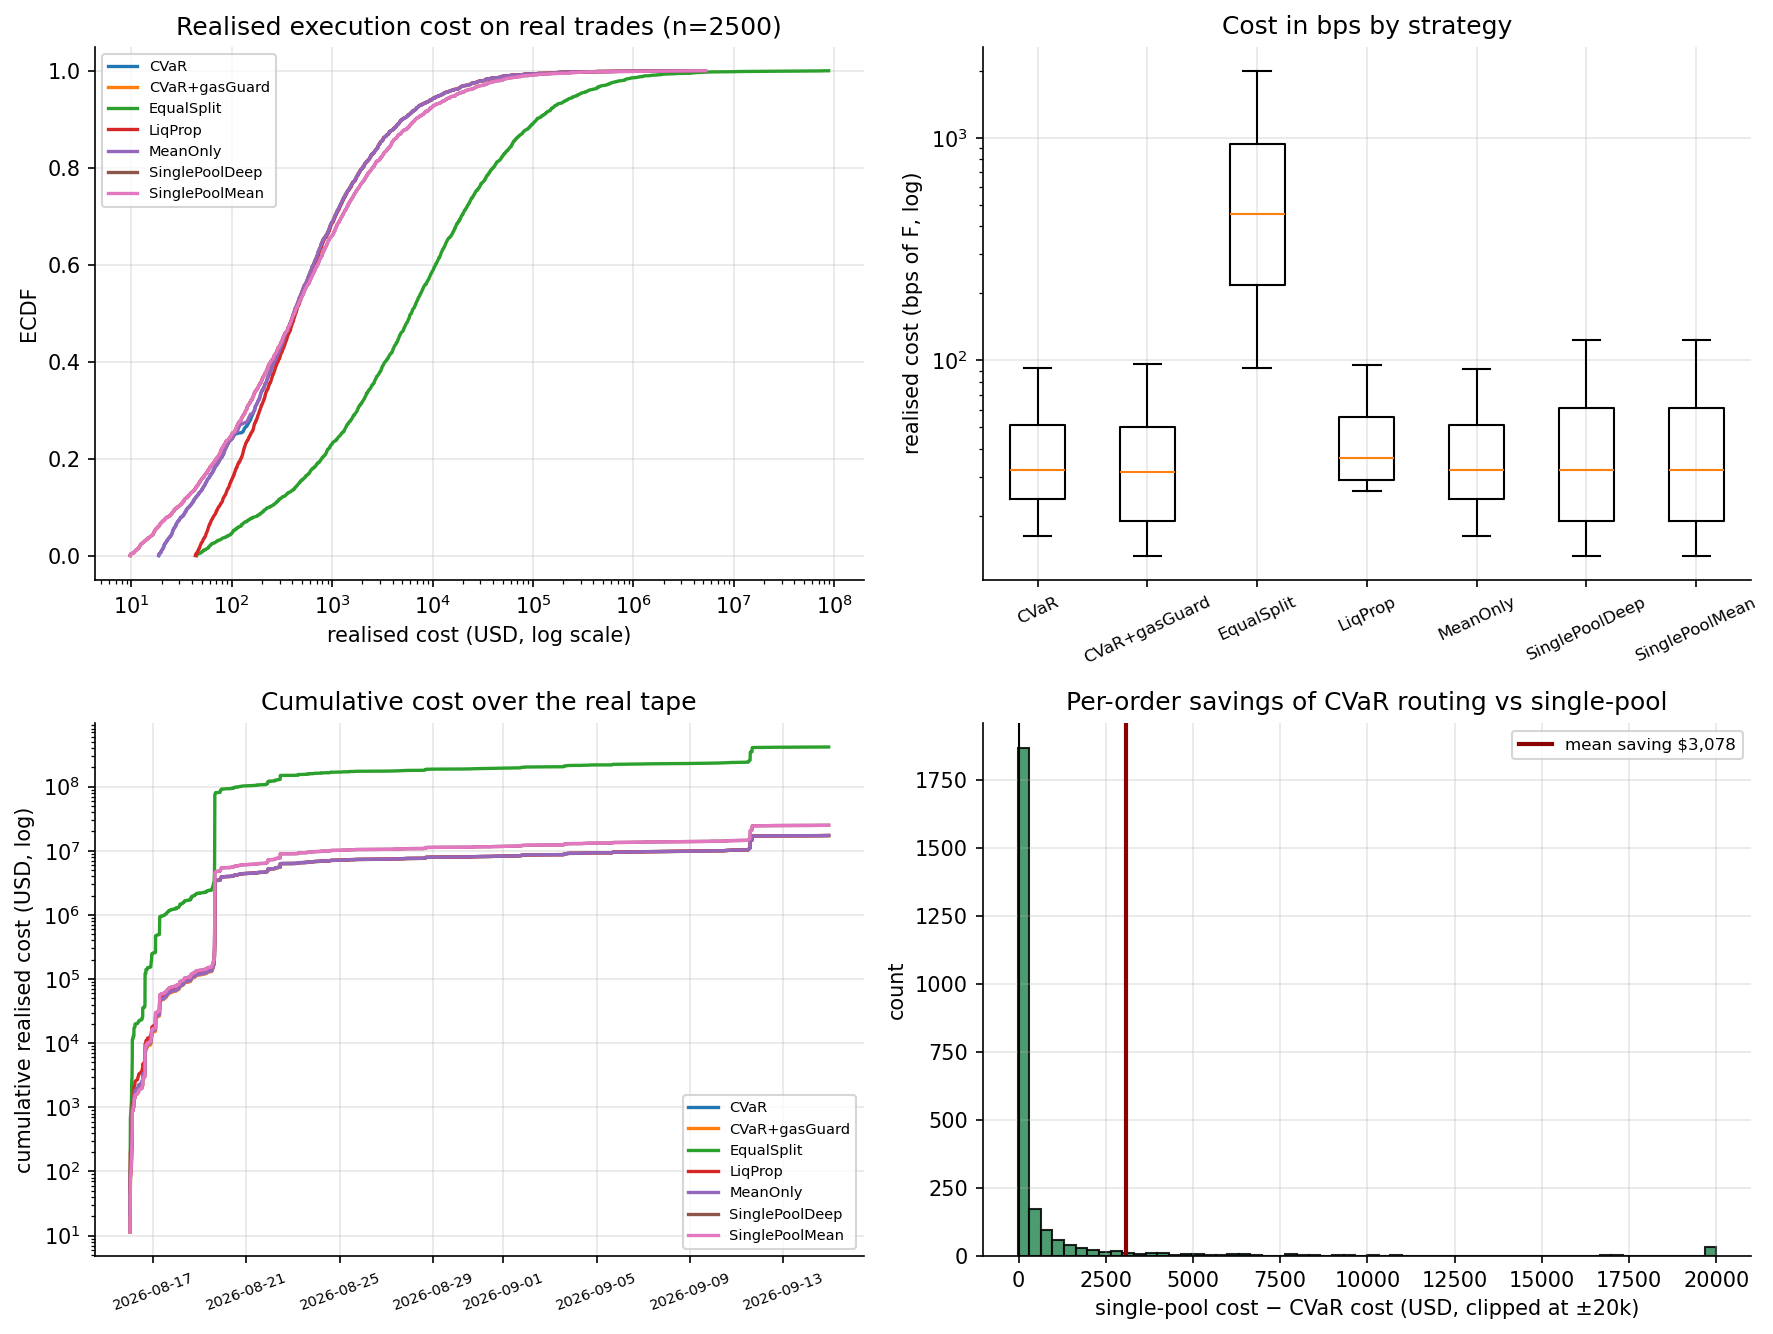
\includegraphics[width=0.98\linewidth]{10_backtest_overall.png}
\caption{Realized execution cost on 2{,}500 real trades.  Top left: empirical CDFs (log
scale).  Top right: cost in bps of $F$.  Bottom left: cumulative cost over the tape.
Bottom right: per-order savings of the \cvar{} router against the best single pool
(mean saving \$3{,}078).}
\label{fig:backtest}
\end{figure}

\begin{figure}[H]
\centering
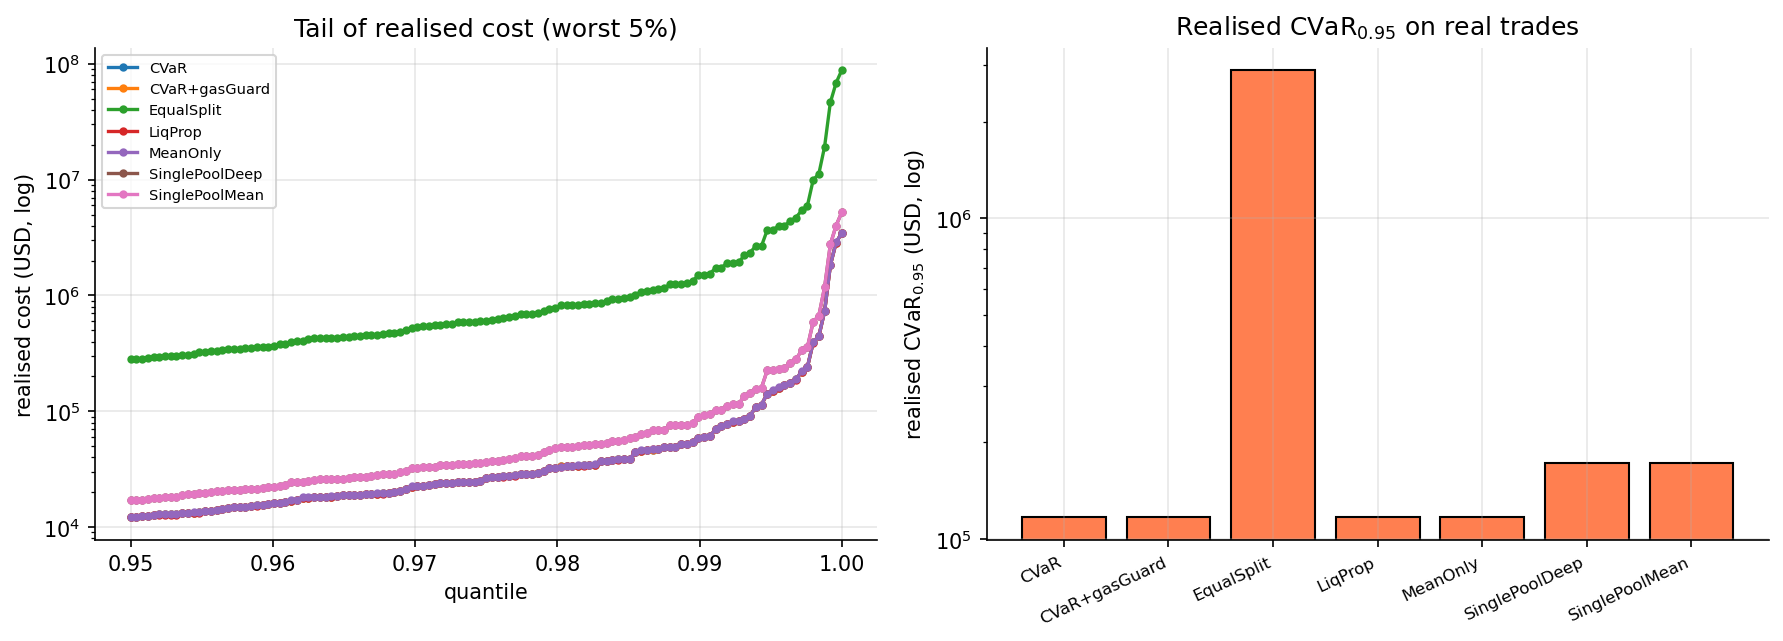
\includegraphics[width=0.92\linewidth]{11_backtest_tail.png}
\caption{Tail behaviour on the real tape.  Left: worst 5\% of realized costs (log scale).
Right: realized $\cvar_{0.95}$ per strategy.}
\label{fig:backtest-tail}
\end{figure}

\subsection{Paired comparison and order-size breakdown}

Table~\ref{tab:paired} compares strategies \emph{per order} (the \cvar{} router is strategy
$A$).  Against the best single pool the router saves \$3{,}078 per order on average and
reduces realized $\cvar_{0.95}$ by \textbf{32.3\%}.  Against mean-only the two are
statistically indistinguishable (51\% win rate, 0.12\% tail difference) --- expected, since
the five real pools have correlated risk factors; see Section~\ref{sec:discussion}.

\begin{table}[H]
\centering
\caption{Paired per-order comparison, \cvar{} router ($A$) vs.\ baseline ($B$), on real
trades.}
\label{tab:paired}
\small
\begin{tabular}{@{}lrrrr@{}}
\toprule
\textbf{vs.} & \textbf{mean saving} & \textbf{win rate of } $A$ & \textbf{tail mean diff.} &
$\cvar$ \textbf{improvement} \\
\midrule
Single-pool best/deepest & \$3{,}078 & 52.2\% & \$29.5 & \textbf{32.3\%} \\
Mean-only & \$8.4 & 51.4\% & \$28.2 & 0.12\% \\
Liquidity-proportional & \$12.9 & 90.5\% & \$174.1 & $-0.13\%$ \\
Equal split & \$159{,}223 & 100\% & $-\$47.4$ & 96.0\% \\
\cvar{} + gas-guard & $-\$6.7$ & 0\% & $-\$29.5$ & 0\% \\
\bottomrule
\end{tabular}
\end{table}

\begin{table}[H]
\centering
\caption{Realized $\cvar_{0.95}$ (USD) by real order size.  The \cvar{} router wins for
$F\gtrsim \$100$k; the gas-guard correctly falls back to a single pool below that.}
\label{tab:by-size}
\small
\begin{tabular}{@{}lrrrr@{}}
\toprule
\textbf{size bucket} & \textbf{\cvar{} router} & \textbf{\cvar{} + gas-guard} &
\textbf{mean-only} & \textbf{single-pool} \\
\midrule
$<\$5$k        & 21.0 & \textbf{12.1} & 21.0 & \textbf{12.1} \\
\$5k--25k       & 41.1 & \textbf{32.9} & 41.2 & \textbf{32.9} \\
\$25k--100k     & 259.1 & \textbf{238.3} & 258.4 & \textbf{238.3} \\
\$100k--500k    & \textbf{3{,}360} & \textbf{3{,}360} & 3{,}367 & 4{,}408 \\
$>\$500$k      & \textbf{724{,}084} & \textbf{724{,}084} & 724{,}827 & 1{,}075{,}235 \\
\bottomrule
\end{tabular}
\end{table}

\begin{figure}[H]
\centering
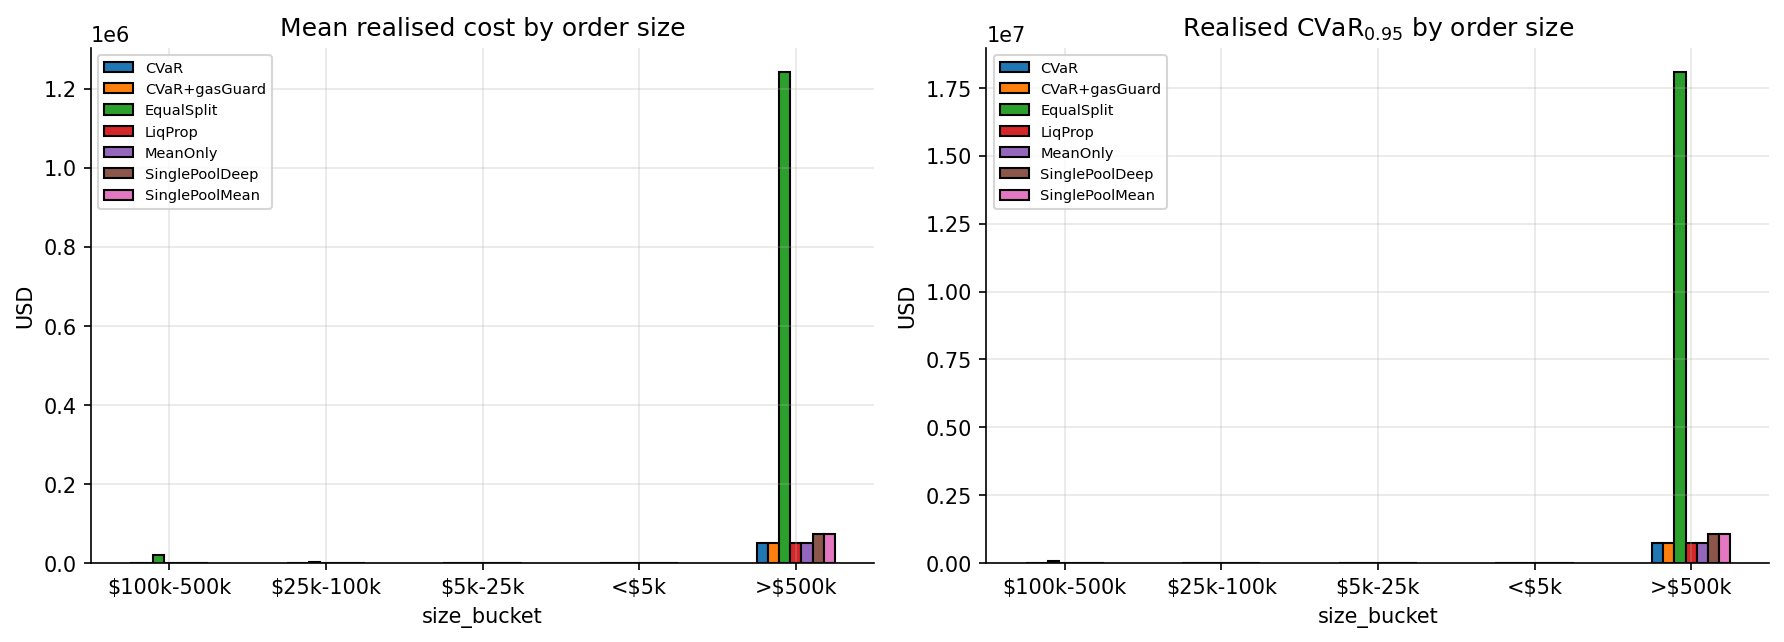
\includegraphics[width=0.98\linewidth]{12_backtest_by_size.png}
\caption{Realized mean (left) and $\cvar_{0.95}$ (right) by real order size.  The crossover
in Table~\ref{tab:by-size} is the out-of-sample counterpart of the F-sweep in
Figure~\ref{fig:sens-F}.}
\label{fig:by-size}
\end{figure}

\subsection{Stressed liquidity days}

On the six worst real liquidity days (top 20\% by mean realized deviation; 564 orders) the
ordering sharpens: the \cvar{} router's tail (\$141{,}198) beats mean-only (\$141{,}556) and
the best single pool (\$196{,}612, $-28\%$).

\begin{table}[H]
\centering
\caption{Realized costs on the worst real liquidity days (564 orders, USD).}
\label{tab:bad-days}
\small
\begin{tabular}{@{}lrrr@{}}
\toprule
\textbf{Strategy} & \textbf{mean} & \textbf{max} & $\cvar_{0.95}$ \\
\midrule
\cvar{} + gas-guard & \textbf{7{,}975} & 2{,}860{,}003 & \textbf{141{,}198} \\
\cvar{} router & 7{,}982 & 2{,}860{,}003 & \textbf{141{,}198} \\
Mean-only & 8{,}002 & 2{,}866{,}724 & 141{,}556 \\
Liquidity-proportional & 8{,}002 & 2{,}861{,}072 & 141{,}217 \\
Single-pool best/deepest & 10{,}967 & 4{,}005{,}525 & 196{,}612 \\
Equal split & 185{,}491 & 68{,}329{,}162 & 3{,}343{,}346 \\
\bottomrule
\end{tabular}
\end{table}

% =====================================================================
\section{Discussion and findings}
\label{sec:discussion}
% =====================================================================

\begin{enumerate}[leftmargin=2.2em]
  \item \textbf{Splitting is worth it for large orders.}  Against the best single pool the
        \cvar{} router cuts realized tail cost by 32.3\% and mean cost by \$3{,}078 per
        order on the real tape; the advantage grows with size ($-22\%$ cost at \$500k,
        $-30\%$ at \$5M in the F-sweep).
  \item \textbf{There is a size threshold} at $F\approx\$100$--$200$k: below it the fixed
        gas of extra pools outweighs the impact saved and one pool is cheaper.  This
        threshold is visible both in-sample (Table~\ref{tab:sens-F}) and out-of-sample
        (Table~\ref{tab:by-size}).  It moves roughly linearly with the gas price.
  \item \textbf{\cvar{} weighting is cheap insurance.}  Against mean-only it is tied out of
        sample (0.12\% tail difference, 51\% win rate) because these five real pools have
        strongly correlated risk factors --- a market-wide liquidity event hits all of them.
        It never gives up more than 0.3\% mean and it is strictly better under higher
        uncertainty (3.5\% tail improvement at twice the observed deviation intensity, and
        0.25\% on the worst real liquidity days).  With more heterogeneous venues
        (e.g.\ pools whose depth is driven by idiosyncratic events) the $\lambda\,\cvar_\alpha$
        term should matter more.
  \item \textbf{The gas-guard is the best practical rule.}  Combining the relaxed \cvar{}
        router with a true-cost fallback to the best single pool (i.e.\ correcting the
        relaxation gap of Lemma~\ref{lem:collapse}) dominates both on the real tape: lowest
        mean cost (\$6{,}902) and lowest cost in bps (48.2).
  \item \textbf{Depth heterogeneity dominates fee heterogeneity at large $F$}, while fee
        tiers matter at small/medium $F$ --- exactly the structure of
        \eqref{eq:cost-m} (linear fee, quadratic impact).  The catastrophic equal-split
        baseline shows what ignoring depth differences costs.
\end{enumerate}

\paragraph{Practical recommendations.}
For orders below \$100k use the best single pool (or the gas-guard rule).  For orders of
\$100k--\$500k use the \cvar{} router with $\lambda\approx1$, $\alpha=0.95$.  For whale
orders (\$5M+) always split; the tail reduction is worth the fee premium.  If you expect
liquidity stress (volatile TVL, high MEV periods) raise $\lambda$ and $\alpha$ --- that is
exactly where the \cvar{} term pays for itself.

% =====================================================================
\section{Review of the earlier project notebooks and corrections}
\label{sec:review}
% =====================================================================

The first version of this project was delivered as two notebooks
(\code{Project\_402111389.ipynb}, \code{Project\_script.ipynb}).  Rewriting the project
surfaced 14 substantive issues; they are listed here for transparency and were all
corrected in the present codebase (which is covered by 32 unit tests).

\begin{table}[H]
\centering
\caption{Issues found in the earlier notebooks and their corrections.}
\label{tab:review}
\small
\begin{tabular}{@{}p{0.5cm}p{6.4cm}p{6.2cm}@{}}
\toprule
\# & \textbf{Issue} & \textbf{Correction} \\
\midrule
1 & ``Real Uniswap data'', ``historical slippage from $\sim$10{,}000 trades'', ``MEV
     vulnerability from Flashbots'' are hardcoded tables or \code{np.random} draws
   & Real downloads only (Binance \code{aggTrades}, DefiLlama TVL); provenance table;
     synthetic quantities removed or labelled \\
2 & Objective $\lambda\,\cvar+(1-\lambda)\,\E[\cdot]+\gamma\, g^{\top}z$ does not match the
     statement $\E[\cdot]+\lambda\,\cvar+\eta\sum z_m$; $g_m z_m$ missing from $C_k$
   & Exact statement implemented \eqref{eq:problem} \\
3 & Markdown constraint ``$z_m\ge\min(x_m,1)$'' is wrong
   & Statement constraints $0\le z_m\le1$, $f_m\le F z_m$; collapse lemma proved
     (Lemma~\ref{lem:collapse}) \\
4 & Liquidity rescaled arbitrarily ($L=\sqrt{\mathrm{TVL}/2}/1000$); costs labelled both USD
     and ETH & Single unit system (USD); $L=\mathrm{TVL}/2$ derived from $xy=k$
     \eqref{eq:L-def} \\
5 & Evaluation helper hardcodes $\alpha=0.95$ and omits gas, biasing the baseline comparison
   & $\alpha$ is a parameter everywhere; all strategies evaluated with the true fixed-gas
     cost \eqref{eq:true-cost} \\
6 & Table of contents promises a theory section that does not exist
   & Derivations and convexity proofs written out (Sections~\ref{sec:model},
     \ref{sec:convexity}) \\
7 & Presentation notes contradict the code (``$\alpha=0.05$'', different baselines)
   & Single source of truth; extras explicitly labelled \\
8 & No out-of-sample evaluation; ``trade history'' is simulated and never used to test the
     model & 2{,}500-order walk-forward backtest on real trades (Section~\ref{sec:backtest}) \\
9 & Deprecated ECOS as primary solver; no solver-status handling
   & CLARABEL primary with SCS fallback and status checks \\
10 & \code{quad\_over\_lin} used in a Python loop over $M\times K$ atoms (slow)
   & DCP-equivalent vectorized form (Section~\ref{sec:convexity}); literal form kept as a
     cross-check reference \\
11 & Evaluation \cvar{} estimator inconsistent with the epigraph used to optimize
   & One estimator, the RU-optimal tail mean, validated against an explicit RU solve in the
     tests \\
12 & Efficient-frontier claims overstated (weighted sums recover supported Pareto points only)
   & Frontier reported descriptively (Section~\ref{sec:sensitivity}) \\
13 & Scenario model (``MEV mixture of uniforms'') not tied to any data
   & Historical resampling of real TVL deviations; trend-inversion defect found and fixed
     (Section~\ref{sec:scenarios}) \\
14 & No tests; no reproducibility guarantees
   & 32 pytest tests (convexity, RU-\cvar{} correctness, DCP, feasibility, no look-ahead,
     backtest smoke) and fixed seeds \\
\bottomrule
\end{tabular}
\end{table}

% =====================================================================
\section{Limitations}
\label{sec:limitations}
% =====================================================================

\begin{itemize}[leftmargin=2.2em]
  \item Realized cost is evaluated with the convex cost model \eqref{eq:cost-m} at the
        \emph{realized real} TVL of the execution day.  A full on-chain replay (pool
        reserves block by block, Uniswap V3 concentrated-liquidity curves) would require an
        archive node or subgraph key.  The model is validated analytically against $xy=k$
        and its cost shape is checked on the real tape (Figure~\ref{fig:impact}).
  \item TVL is observed at daily granularity (DefiLlama); intra-day liquidity variation is
        unobserved.
  \item Gas costs are estimated (swap gas units $\times$ 20 gwei $\times$ the real ETH
        price).  The F-sweep threshold moves roughly linearly with the gas price; the
        qualitative conclusions hold between 5 and 50 gwei.
  \item Uniswap V3 concentrated liquidity and Curve-style amplifiers are approximated by the
        constant-product index $L=\mathrm{TVL}/2$; a per-pool efficiency factor $\kappa_m$
        ($L_m=\kappa_m\,\mathrm{TVL}_m/2$) is the natural refinement.
  \item The five pools trade the same pair and have correlated risk factors, which is why
        \cvar{} weighting and mean-only are nearly tied out of sample
        (Section~\ref{sec:discussion}).
\end{itemize}

% =====================================================================
\section{Conclusions}
% =====================================================================

We studied the convex \cvar{} order-routing problem of the project statement end to end,
with real market data and real trades.  The cost model $a_m f_m + b_m f_m^2/L_m$ is the
second-order expansion of the exact constant-product cost, the \cvar{} term is the
Rockafellar--Uryasev epigraph, and the whole problem is DCP and DPP-compliant in CVXPY
(131 variables and 251 constraints in the base case, solved in 14.6 ms).  On real trades the
router reduces realized tail cost by 32.3\% versus the best single pool for orders above
\$100--200k, and the \cvar{} term itself provides cheap insurance against liquidity stress.
The prescribed $z_m$ relaxation collapses to allocation shares (Lemma~\ref{lem:collapse}),
which prices splitting correctly for large orders but over-splits small ones --- a gap that
the gas-guard rule closes.  All computations are reproducible from the accompanying code
and the 32-test suite.

% =====================================================================
\begin{thebibliography}{9}
\bibitem{adams2021uniswap}
H.~Adams, N.~Zinsmeister, N.~Salem, R.~Keefer, and D.~Robinson.
\emph{Uniswap v2 Core}. Whitepaper, Uniswap, 2021.

\bibitem{angeris2022optimal}
G.~Angeris, T.~Chitra, A.~Evans, and S.~Boyd.
\emph{Optimal Routing for Constant Function Market Makers}.
arXiv:2101.08020v4, 2022.

\bibitem{boyd2004convex}
S.~Boyd and L.~Vandenberghe.
\emph{Convex Optimization}. Cambridge University Press, 2004.

\bibitem{daian2020flash}
P.~Daian, S.~Goldfeder, T.~Kell, Y.~Li, X.~Zhao, I.~Bentov, L.~Breidenbach, and A.~Juels.
\emph{Flash Boys 2.0: Frontrunning in Decentralized Exchanges, Miner Extractable Value, and
Consensus Instability}. IEEE Symposium on Security and Privacy, 2020.

\bibitem{rockafellar2000optimization}
R.~T.~Rockafellar and S.~Uryasev.
\emph{Optimization of Conditional Value-at-Risk}.
Journal of Risk, 2(3):21--41, 2000.

\bibitem{data-sources}
Binance Vision (\url{https://data.binance.vision}) aggregated trades and klines; DefiLlama
Yields API (\url{https://yields.llama.fi}) real DEX pool TVL histories.
\end{thebibliography}

% =====================================================================
\appendix
\section{Complete result tables}
\label{app:tables}

Full-precision versions of every table in the report (source: \code{results/tables/*.csv}).

\begin{landscape}
\begin{table}[H]
\centering
\caption*{\textbf{A.1} Base-case allocation (\code{base\_case\_allocation.csv})}
\scriptsize
\begin{tabular}{@{}llrrrrrr@{}}
\toprule
pool & project & fee & $L$ (USD) & gas (USD) & $f_m$ (USD) & share & $z_m$ \\
\midrule
uniswap-v3 USDC-WETH (0.05\%) & uniswap-v3 & 0.0005 & 53{,}470{,}826.5 & 9.130305 &
184{,}531.306701 & 0.7381252268 & 0.7381253801 \\
uniswap-v3 USDC-WETH (0.3\%) & uniswap-v3 & 0.0030 & 15{,}054{,}635.5 & 9.130305 &
33{,}374.384791 & 0.1334975392 & 0.1334976983 \\
uniswap-v2 USDC-WETH & uniswap-v2 & 0.0030 & 10{,}083{,}282.5 & 7.402950 &
25{,}712.309358 & 0.1028488574 & 0.1028488733 \\
uniswap-v3 USDC-WETH (0.01\%) & uniswap-v3 & 0.0001 & 1{,}825{,}237.5 & 9.130305 &
6{,}103.778741 & 0.0244151150 & 0.0244151058 \\
sushiswap USDC-WETH & sushiswap & 0.0030 & 137{,}919.5 & 7.402950 &
278.220409 & 0.0011128816 & 0.0011132425 \\
\bottomrule
\end{tabular}
\end{table}

\begin{table}[H]
\centering
\caption*{\textbf{A.2} In-sample baselines with full precision
(\code{baselines\_insample.csv}; allocations as $f_m$ per pool)}
\scriptsize
\begin{tabular}{@{}lrrrrrr@{}}
\toprule
strategy & mean\_cost & VaR\_0.95 & CVaR\_0.95 & max\_cost & n\_pools & allocation ($f_m$) \\
\midrule
CVaR (ours) & 1194.390969 & 1266.429865 & 1308.863246 & 1442.988014 & 4 &
184531.31, 33374.38, 25712.31, 6103.78, 278.22 \\
MeanOnly (lambda=0) & 1191.322151 & 1278.213612 & 1317.935454 & 1450.714492 & 4 &
191036.28, 29255.82, 23342.25, 6164.36, 201.29 \\
SinglePoolBest (mean) & 1389.490881 & 1581.269654 & 1628.128837 & 1785.717417 & 1 &
250000.00, 0.00, 0.00, 0.00, 0.00 \\
SinglePoolDeep (max L) & 1389.490881 & 1581.269654 & 1628.128837 & 1785.717417 & 1 &
250000.00, 0.00, 0.00, 0.00, 0.00 \\
Equal split (extra) & 34882.787733 & 48487.343804 & 48563.264796 & 48600.492721 & 5 &
50000.00, 50000.00, 50000.00, 50000.00, 50000.00 \\
Liq-proportional (extra) & 1218.106836 & 1274.319576 & 1314.780870 & 1447.978364 & 4 &
(see CSV) \\
\bottomrule
\end{tabular}
\end{table}

\begin{table}[H]
\centering
\caption*{\textbf{A.3} Sensitivity over $\alpha$ (\code{sensitivity\_alpha.csv})}
\scriptsize
\begin{tabular}{@{}rrrrrrrr@{}}
\toprule
alpha & mean\_cost & CVaR\_eval & CVaR\_own\_alpha & VaR\_eval & max\_cost &
solve\_time\_ms & n\_active \\
\midrule
0.80 & 1194.295564 & 1309.130539 & 1267.539564 & 1266.278507 & 1443.883844 & 970.83 & 4 \\
0.90 & 1195.197096 & 1308.237820 & 1285.119699 & 1265.072514 & 1443.134113 & 890.27 & 4 \\
0.95 & 1194.390969 & 1308.863246 & 1308.863246 & 1266.429865 & 1442.988014 & 14.10 & 4 \\
0.99 & 1193.386916 & 1310.976176 & 1418.813881 & 1270.172532 & 1443.183540 & 965.96 & 4 \\
\bottomrule
\end{tabular}
\end{table}

\begin{table}[H]
\centering
\caption*{\textbf{A.4} Sensitivity over $F$ (\code{sensitivity\_size.csv})}
\scriptsize
\begin{tabular}{@{}rrrrrrrrr@{}}
\toprule
F & n\_active & mean\_cost & mean\_bps & CVaR & CVaR\_bps & max\_cost & single\_pool\_mean &
solve\_ms \\
\midrule
1{,}000 & 2 & 18.710901 & 187.109 & 18.730892 & 187.309 & 18.733653 & 9.650391 & 12.59 \\
5{,}000 & 2 & 21.129163 & 42.258 & 21.220958 & 42.442 & 21.310254 & 12.132449 & 15.86 \\
10{,}000 & 2 & 25.031058 & 25.031 & 25.385296 & 25.385 & 25.683119 & 16.139203 & 13.36 \\
50{,}000 & 2 & 91.331315 & 18.266 & 100.312816 & 20.063 & 106.930806 & 84.345388 & 13.09 \\
100{,}000 & 4 & 279.440146 & 27.944 & 305.583062 & 30.558 & 327.595289 & 259.987744 & 12.27 \\
500{,}000 & 4 & 4111.986622 & 82.240 & 4520.938558 & 90.419 & 5063.431164 & 5280.573323 & 14.15 \\
1{,}000{,}000 & 4 & 15186.246380 & 151.862 & 16741.615515 & 167.416 & 18895.356569 &
20594.900044 & 13.49 \\
5{,}000{,}000 & 4 & 354731.150 & 709.462 & 393343.933 & 786.688 & 446799.006 &
504653.361 & 13.39 \\
\bottomrule
\end{tabular}
\end{table}

\begin{table}[H]
\centering
\caption*{\textbf{A.5} Sensitivity over the uncertainty intensity
(\code{sensitivity\_delta.csv})}
\scriptsize
\begin{tabular}{@{}rlrrrrr@{}}
\toprule
delta\_scale & strategy & mean\_cost & CVaR & VaR & max\_cost & n\_active \\
\midrule
0.0 & CVaR & 1109.240260 & 1109.240260 & 1109.240260 & 1109.240260 & 4 \\
0.0 & MeanOnly & 1109.240263 & 1109.240263 & 1109.240263 & 1109.240263 & 4 \\
0.5 & CVaR & 1145.969296 & 1196.428773 & 1179.882896 & 1247.503626 & 4 \\
0.5 & MeanOnly & 1145.363151 & 1198.210385 & 1182.233474 & 1248.871257 & 4 \\
1.0 & CVaR & 1194.390969 & 1308.863246 & 1266.429865 & 1442.988014 & 4 \\
1.0 & MeanOnly & 1191.322151 & 1317.935454 & 1278.213612 & 1450.714492 & 4 \\
1.5 & CVaR & 1263.619266 & 1471.942944 & 1372.693909 & 1742.131090 & 4 \\
1.5 & MeanOnly & 1251.067408 & 1508.657848 & 1409.704947 & 1763.636284 & 4 \\
2.0 & CVaR & 1313.690184 & 1629.260321 & 1499.479358 & 2156.443794 & 4 \\
2.0 & MeanOnly & 1295.303969 & 1688.706059 & 1561.441004 & 2235.946568 & 4 \\
\bottomrule
\end{tabular}
\end{table}

\begin{table}[H]
\centering
\caption*{\textbf{A.6} Efficient frontier in $\lambda$ (\code{frontier.csv})}
\scriptsize
\begin{tabular}{@{}rrrr@{}}
\toprule
lam & mean\_cost & CVaR & max\_cost \\
\midrule
0.00 & 1191.322151 & 1317.935454 & 1450.714492 \\
0.10 & 1191.424624 & 1315.855180 & 1448.783250 \\
0.25 & 1191.805747 & 1313.608113 & 1446.765475 \\
0.50 & 1192.679644 & 1311.236700 & 1444.770668 \\
0.75 & 1193.570670 & 1309.795581 & 1443.655545 \\
1.00 & 1194.390969 & 1308.863246 & 1442.988014 \\
1.50 & 1195.763154 & 1307.747480 & 1442.296888 \\
2.00 & 1196.812443 & 1307.148793 & 1442.006646 \\
4.00 & 1199.288861 & 1306.247464 & 1441.820338 \\
8.00 & 1201.205452 & 1305.895697 & 1441.988144 \\
\bottomrule
\end{tabular}
\end{table}

\begin{table}[H]
\centering
\caption*{\textbf{A.7} Scalability (\code{scalability.csv})}
\scriptsize
\begin{tabular}{@{}rrrrllrr@{}}
\toprule
M & K & cold\_ms & solve\_ms & solver & status & n\_variables & n\_constraints \\
\midrule
5 & 50 & 328.10 & 5.56 & CLARABEL & optimal & 61 & 111 \\
5 & 100 & 631.41 & 10.82 & CLARABEL & optimal & 111 & 211 \\
5 & 200 & 2665.52 & 23.30 & CLARABEL & optimal & 211 & 411 \\
10 & 50 & 338.24 & 8.57 & CLARABEL & optimal & 71 & 121 \\
10 & 100 & 1423.73 & 14.86 & CLARABEL & optimal & 121 & 221 \\
10 & 200 & 10028.42 & 38.52 & CLARABEL & optimal & 221 & 421 \\
20 & 50 & 670.62 & 15.04 & CLARABEL & optimal & 91 & 141 \\
20 & 100 & 4040.91 & 28.56 & CLARABEL & optimal & 141 & 241 \\
20 & 200 & 33152.09 & 66.53 & CLARABEL & optimal & 241 & 441 \\
\bottomrule
\end{tabular}
\end{table}

\begin{table}[H]
\centering
\caption*{\textbf{A.8} Backtest summary (\code{backtest\_summary.csv}; USD and bps)}
\scriptsize
\begin{tabular}{@{}lrrrrrrrr@{}}
\toprule
strategy & mean & median & std & min & max & VaR\_0.95 & CVaR\_0.95 & bps\_mean \\
\midrule
CVaR & 6908.854 & 414.436 & 99522.358 & 18.693 & 3469555.509 & 12178.141 & 117000.348 &
50.434 \\
CVaR+gasGuard & 6902.123 & 414.436 & 99522.815 & 9.672 & 3469555.509 & 12178.141 &
117000.348 & 48.166 \\
EqualSplit & 166131.66 & 6161.68 & 2481795.77 & --- & 88266269.86 & 280810.07 &
2895020.18 & 922.56 \\
LiqProp & 6921.76 & 433.91 & 99410.84 & --- & 3463138.28 & 12172.87 & 116847.57 &
57.38 \\
MeanOnly & 6917.26 & 414.02 & 99609.72 & --- & 3469956.95 & 12205.12 & 117139.64 &
50.39 \\
SinglePoolDeep & 9987.30 & 422.07 & 147045.75 & --- & 5245924.78 & 17037.35 & 172781.05 &
60.32 \\
SinglePoolMean & 9987.30 & 422.07 & 147045.75 & --- & 5245924.78 & 17037.35 & 172781.05 &
60.32 \\
\bottomrule
\end{tabular}
\end{table}

\begin{table}[H]
\centering
\caption*{\textbf{A.9} Paired comparison (\code{backtest\_paired.csv})}
\scriptsize
\begin{tabular}{@{}lrrrrrr@{}}
\toprule
vs & mean\_diff\_A-B & median\_diff & win\_rate\_A & tie\_rate & mean\_diff\_worst\_tail &
CVaR\_improvement\_pct \\
\midrule
CVaR+gasGuard & 6.731 & 0.000 & 0.000 & 0.530 & 29.537 & 0.000 \\
EqualSplit & -159222.807 & -5740.615 & 1.000 & 0.000 & -47.420 & 95.959 \\
LiqProp & -12.903 & -20.521 & 0.905 & 0.000 & 174.063 & -0.131 \\
MeanOnly & -8.410 & -0.001 & 0.514 & 0.000 & 28.220 & 0.119 \\
SinglePoolDeep & -3078.450 & -6.460 & 0.522 & 0.000 & 29.537 & 32.284 \\
SinglePoolMean & -3078.450 & -6.460 & 0.522 & 0.000 & 29.537 & 32.284 \\
\bottomrule
\end{tabular}
\end{table}

\begin{table}[H]
\centering
\caption*{\textbf{A.10} Realized $\cvar_{0.95}$ by order size
(\code{backtest\_by\_size.csv})}
\scriptsize
\begin{tabular}{@{}llrrr@{}}
\toprule
size\_bucket & strategy & mean & VaR\_0.95 & CVaR\_0.95 \\
\midrule
<\$5k & CVaR & 19.9236 & 21.0201 & 21.0488 \\
<\$5k & CVaR+gasGuard & 10.9317 & 12.0637 & 12.0783 \\
<\$5k & EqualSplit & 52.1545 & 59.5509 & 59.8816 \\
<\$5k & LiqProp & 45.9584 & 48.5510 & 48.5889 \\
<\$5k & MeanOnly & 19.9183 & 21.0163 & 21.0469 \\
<\$5k & SinglePoolDeep & 10.9317 & 12.0637 & 12.0783 \\
<\$5k & SinglePoolMean & 10.9317 & 12.0637 & 12.0783 \\
\$5k--25k & CVaR & 29.6665 & 40.3611 & 41.1467 \\
\$5k--25k & CVaR+gasGuard & 21.0099 & 32.3794 & 32.8652 \\
\$5k--25k & EqualSplit & 149.3947 & 276.7313 & 283.8633 \\
\$5k--25k & LiqProp & 62.4591 & 78.4141 & 80.5542 \\
\$5k--25k & MeanOnly & 29.6672 & 40.3698 & 41.1514 \\
\$5k--25k & SinglePoolDeep & 21.0099 & 32.3794 & 32.8652 \\
\$5k--25k & SinglePoolMean & 21.0099 & 32.3794 & 32.8652 \\
\$25k--100k & CVaR & 134.2674 & 251.1329 & 259.0577 \\
\$25k--100k & CVaR+gasGuard & 117.2239 & 228.4130 & 238.3395 \\
\$25k--100k & EqualSplit & 1479.4357 & 3132.1709 & 3298.8488 \\
\$25k--100k & LiqProp & 167.3282 & 271.8151 & 281.3645 \\
\$25k--100k & MeanOnly & 132.1712 & 249.9532 & 258.4145 \\
\$25k--100k & SinglePoolDeep & 117.2239 & 228.4130 & 238.3395 \\
\$25k--100k & SinglePoolMean & 117.2239 & 228.4130 & 238.3395 \\
\$100k--500k & CVaR & 1100.3640 & 2993.6627 & 3360.2943 \\
\$100k--500k & CVaR+gasGuard & 1098.6298 & 2993.6627 & 3360.2943 \\
\$100k--500k & EqualSplit & 20764.2643 & 63063.5614 & 71024.0738 \\
\$100k--500k & LiqProp & 1116.2164 & 3007.0827 & 3366.2225 \\
\$100k--500k & MeanOnly & 1101.3868 & 2995.5568 & 3367.3633 \\
\$100k--500k & SinglePoolDeep & 1328.8452 & 3911.8398 & 4407.4650 \\
\$100k--500k & SinglePoolMean & 1328.8452 & 3911.8398 & 4407.4650 \\
>\$500k & CVaR & 50537.6631 & 109038.2232 & 724084.3669 \\
>\$500k & CVaR+gasGuard & 50537.6631 & 109038.2232 & 724084.3669 \\
>\$500k & EqualSplit & 1241151.601 & 2668697.5895 & 18072655.1243 \\
>\$500k & LiqProp & 50476.2172 & 108917.0926 & 723208.3286 \\
>\$500k & MeanOnly & 50605.5996 & 109213.0126 & 724826.7632 \\
>\$500k & SinglePoolDeep & 74236.0676 & 157331.7937 & 1075235.3209 \\
>\$500k & SinglePoolMean & 74236.0676 & 157331.7937 & 1075235.3209 \\
\bottomrule
\end{tabular}
\end{table}

\begin{table}[H]
\centering
\caption*{\textbf{A.11} Stressed liquidity days (\code{backtest\_bad\_days.csv}; 564
orders on 6 days, severity threshold 0.174)}
\scriptsize
\begin{tabular}{@{}lrrrrr@{}}
\toprule
strategy & n & mean & median & max & CVaR\_0.95 \\
\midrule
CVaR & 564 & 7981.947 & 273.6289 & 2860002.9964 & 141197.5388 \\
CVaR+gasGuard & 564 & 7974.9812 & 255.8630 & 2860002.9964 & 141197.5388 \\
EqualSplit & 564 & 185490.8442 & 3588.9970 & 68329161.7126 & 3343345.7963 \\
LiqProp & 564 & 8001.8675 & 292.1496 & 2861072.0731 & 141217.0616 \\
MeanOnly & 564 & 8001.5925 & 273.1405 & 2866723.5747 & 141556.0091 \\
SinglePoolDeep & 564 & 10967.3715 & 255.8630 & 4005524.9586 & 196612.1351 \\
SinglePoolMean & 564 & 10967.3715 & 255.8630 & 4005524.9586 & 196612.1351 \\
\bottomrule
\end{tabular}
\end{table}

\begin{table}[H]
\centering
\caption*{\textbf{A.12} Tape impact fit (\code{impact\_fit.json})}
\small
\begin{tabular}{@{}lr@{}}
\toprule
$\hat a$ (linear, bps scale) & $1.2795\times 10^{-4}$ \\
$\hat b$ (quadratic) & $-1.0417\times 10^{-9}$ \\
bin-mean $R^{2}$ & 0.9196 \\
observations (1s clips) & 53{,}68 \\
size bins & 18 \\
Spearman(size, cost) & 0.8803 \\
bps at smallest / largest bin & 0.5446 \,/\, 0.7120 \\
\bottomrule
\end{tabular}
\end{table}

\begin{table}[H]
\centering
\caption*{\textbf{A.13} Base-case meta (\code{base\_case\_meta.json})}
\small
\begin{tabular}{@{}lr@{}}
\toprule
$M$ / $K$ & 5 / 120 \\
$F$ (USD) & 250{,}000 \\
$\alpha$ / $\lambda$ / $\eta$ & 0.95 / 1.0 / 0.0 \\
reference date & 2026-08-31 \\
solver / status & CLARABEL / optimal \\
solve time (ms) & 14.604 \\
optimal objective & 2{,}436.762 \\
mean scenario cost & 1{,}194.391 \\
$\cvar_{0.95}$ & 1{,}308.863 \\
variables / constraints & 131 / 251 \\
\bottomrule
\end{tabular}
\end{table}

\begin{table}[H]
\centering
\caption*{\textbf{A.14} Real trade-tape statistics (\code{trade\_stats.json})}
\small
\begin{tabular}{@{}lr@{}}
\toprule
real trades parsed & 25{,}544{,}800 \\
aggressive sell notional (USD) & 11{,}982{,}345{,}569 \\
aggressive buy notional (USD) & 12{,}167{,}878{,}134 \\
median single trade (USD) & 31.76 \\
mean single trade (USD) & 945.41 \\
95th pct single trade (USD) & 4{,}310.53 \\
99.9th pct single trade (USD) & 57{,}937.89 \\
\bottomrule
\end{tabular}
\end{table}
\end{landscape}

\section{Raw console output: in-sample experiments}
\label{app:log03}
\lstinputlisting[style=logstyle,caption={Full console output of
\code{scripts/03\_solve\_and\_analyze.py} (base case, baselines, sensitivity sweeps,
frontier, scalability).}]{appendix_files/output_03_solve.log}

\section{Raw console output: real-trade backtest}
\label{app:log04}
\lstinputlisting[style=logstyle,caption={Full console output of
\code{scripts/04\_backtest\_real\_trades.py}.}]{appendix_files/output_04_backtest.log}

\section{Test suite}
\label{app:tests}
\lstinputlisting[style=logstyle,caption={\code{pytest -v}: 32 tests covering numerical
convexity, RU-\cvar{} correctness against an explicit epigraph solve, DCP compliance and
feasibility of the formulation, scenario no-look-ahead and trend-inversion regression, and
an end-to-end backtest smoke test.}]{appendix_files/output_tests.log}

\section{Key code excerpts}
\label{app:code}

\subsection*{E.1 The DPP formulation (\code{src/amm\_cvar/optimizer.py})}
\begin{lstlisting}[style=pystyle]
slip = [cp.sum_squares(cp.multiply(self.p_slip[:, k], self.x)) for k in range(K)]
self.C_k = [self.p_a @ self.x + slip[k] + self.p_g @ self.z for k in range(K)]
C_vec = cp.hstack(self.C_k)
mean_expr = (1.0 / K) * cp.sum(C_vec)
cons = [cp.sum(self.x) == 1.0, self.z <= 1.0, self.x <= self.z]
if lam > 0:
    self.t = cp.Variable(name="t")
    self.u = cp.Variable(K, nonneg=True, name="u")
    cons.append(self.u >= C_vec - self.t)
    cvar_expr = self.t + (1.0 / ((1.0 - alpha) * K)) * cp.sum(self.u)
    obj = mean_expr + lam * cvar_expr + self.p_eta * cp.sum(self.z)
\end{lstlisting}

\subsection*{E.2 Scenario generation (\code{src/amm\_cvar/scenarios.py})}
\begin{lstlisting}[style=pystyle]
G = np.exp(np.mean(np.log(np.maximum(L_hist, 1e-9)), axis=0))   # typical level (M,)
for k in range(K_all):
    day_state = L_hist[-(k + 2)]      # day before the reference day
    deltas_all[:, k] = np.clip(1.0 - day_state / G, 0.0, delta_bar)
deltas_all = np.clip(deltas_all * delta_scale, 0.0, delta_bar)
# keep the 24 worst shortfall days + a seeded uniform sample of the rest
\end{lstlisting}

\subsection*{E.3 Walk-forward loop (\code{src/amm\_cvar/backtest.py})}
\begin{lstlisting}[style=pystyle]
for i, row in orders.iterrows():
    day = row["day"]
    if day not in scen_cache:                       # strictly past data only
        scen_cache[day] = trailing_scenarios(tvl, day, window=window)
        real_cache[day] = realized_state(tvl, day)  # actual next state
    allocs = _strategy_allocations(row["F"], scen_cache[day], a, b, gas, ...)
    for name, f in allocs.items():
        cost = true_execution_cost(f, real_cache[day]["L_real"], a, b, gas)
        records.append({"ts": row["ts"], "F": row["F"], "strategy": name,
                        "realized_cost": cost, ...})
\end{lstlisting}

\subsection*{E.4 True evaluation cost with fixed gas (\code{src/amm\_cvar/cost\_model.py})}
\begin{lstlisting}[style=pystyle]
def true_execution_cost(f, L, a, b, gas, used_tol=0.0) -> float:
    used = f > used_tol
    fee = float(a @ f)
    impact = float(np.sum(b[used] * f[used] ** 2 / L[used]))
    g = float(gas[used].sum())
    return fee + impact + g
\end{lstlisting}

\section{Reproducibility and data manifest}
\label{app:repro}

Everything is reproducible from the \code{amm\_cvar/} codebase (fixed seed 42):

\begin{lstlisting}[style=logstyle]
cd amm_cvar
pip install -r requirements.txt
PYTHONPATH=src python scripts/01_download_data.py        # real data -> data/raw
PYTHONPATH=src python scripts/02_prepare_data.py         # tape -> orders, pools
PYTHONPATH=src python scripts/03_solve_and_analyze.py    # base case + sensitivities
PYTHONPATH=src python scripts/04_backtest_real_trades.py # 2,500-order backtest
PYTHONPATH=src python -m pytest tests -q                 # 32 tests
\end{lstlisting}

\textbf{Trade tape manifest.}  30 daily Binance ETH/USDT \code{aggTrades} archives,
2026-08-16 to 2026-09-14 (ZIP files 2.3--37.1 MB each, 382.7 MB total), cached under
\code{data/raw/aggtrades/ETHUSDT/}.  One-hour klines cover 2024-04 to 2026-09 (29 monthly
archives).

\textbf{Pool IDs (DefiLlama).}
\code{665dc8bc-...} Uniswap V3 USDC-WETH 0.05\%;
\code{49717ee2-...} Uniswap V3 USDC-WETH 0.3\%;
\code{702fff16-...} Uniswap V2 USDC-WETH;
\code{8b3ed515-...} Uniswap V3 USDC-WETH 0.01\%;
\code{966e2c65-...} SushiSwap USDC-WETH.

\textbf{Unit conversions.}  $L_m=\mathrm{TVL}_m/2$ (USD); $a_m=\phi_m$; $b_m=1$;
$g_m$ = swap gas units (V3 185k, V2/Sushi 150k) $\times$ 20 gwei $\times$ \$2{,}467.65.

\textbf{Randomness.}  All sampling (scenario subsetting, backtest order stratification)
uses \code{numpy.random.default\_generator(42)}.

\end{document}
